\documentclass[man,floatsintext]{apa6}
\usepackage{lmodern}
\usepackage{amssymb,amsmath}
\usepackage{ifxetex,ifluatex}
\usepackage{fixltx2e} % provides \textsubscript
\ifnum 0\ifxetex 1\fi\ifluatex 1\fi=0 % if pdftex
  \usepackage[T1]{fontenc}
  \usepackage[utf8]{inputenc}
\else % if luatex or xelatex
  \ifxetex
    \usepackage{mathspec}
  \else
    \usepackage{fontspec}
  \fi
  \defaultfontfeatures{Ligatures=TeX,Scale=MatchLowercase}
\fi
% use upquote if available, for straight quotes in verbatim environments
\IfFileExists{upquote.sty}{\usepackage{upquote}}{}
% use microtype if available
\IfFileExists{microtype.sty}{%
\usepackage{microtype}
\UseMicrotypeSet[protrusion]{basicmath} % disable protrusion for tt fonts
}{}
\usepackage{hyperref}
\hypersetup{unicode=true,
            pdftitle={Seeking social information during language comprehension and word learning},
            pdfauthor={Kyle MacDonald, Elizabeth Swanson, \& Michael C. Frank},
            pdfkeywords={eye movements; word learning; language comprehension;
information-seeking; gaze following},
            pdfborder={0 0 0},
            breaklinks=true}
\urlstyle{same}  % don't use monospace font for urls
\usepackage{graphicx,grffile}
\makeatletter
\def\maxwidth{\ifdim\Gin@nat@width>\linewidth\linewidth\else\Gin@nat@width\fi}
\def\maxheight{\ifdim\Gin@nat@height>\textheight\textheight\else\Gin@nat@height\fi}
\makeatother
% Scale images if necessary, so that they will not overflow the page
% margins by default, and it is still possible to overwrite the defaults
% using explicit options in \includegraphics[width, height, ...]{}
\setkeys{Gin}{width=\maxwidth,height=\maxheight,keepaspectratio}
\IfFileExists{parskip.sty}{%
\usepackage{parskip}
}{% else
\setlength{\parindent}{0pt}
\setlength{\parskip}{6pt plus 2pt minus 1pt}
}
\setlength{\emergencystretch}{3em}  % prevent overfull lines
\providecommand{\tightlist}{%
  \setlength{\itemsep}{0pt}\setlength{\parskip}{0pt}}
\setcounter{secnumdepth}{0}
% Redefines (sub)paragraphs to behave more like sections
\ifx\paragraph\undefined\else
\let\oldparagraph\paragraph
\renewcommand{\paragraph}[1]{\oldparagraph{#1}\mbox{}}
\fi
\ifx\subparagraph\undefined\else
\let\oldsubparagraph\subparagraph
\renewcommand{\subparagraph}[1]{\oldsubparagraph{#1}\mbox{}}
\fi

%%% Use protect on footnotes to avoid problems with footnotes in titles
\let\rmarkdownfootnote\footnote%
\def\footnote{\protect\rmarkdownfootnote}


  \title{Seeking social information during language comprehension and word
learning}
    \author{Kyle MacDonald\textsuperscript{1}, Elizabeth Swanson\textsuperscript{1},
\& Michael C. Frank\textsuperscript{1}}
    \date{}
  
\shorttitle{Integrating social and statistical information}
\affiliation{
\vspace{0.5cm}
\textsuperscript{1} Stanford University}
\keywords{eye movements; word learning; language comprehension; information-seeking; gaze following\newline\indent Word count: X}
\usepackage{csquotes}
\usepackage{upgreek}
\captionsetup{font=singlespacing,justification=justified}

\usepackage{longtable}
\usepackage{lscape}
\usepackage{multirow}
\usepackage{tabularx}
\usepackage[flushleft]{threeparttable}
\usepackage{threeparttablex}

\newenvironment{lltable}{\begin{landscape}\begin{center}\begin{ThreePartTable}}{\end{ThreePartTable}\end{center}\end{landscape}}

\makeatletter
\newcommand\LastLTentrywidth{1em}
\newlength\longtablewidth
\setlength{\longtablewidth}{1in}
\newcommand{\getlongtablewidth}{\begingroup \ifcsname LT@\roman{LT@tables}\endcsname \global\longtablewidth=0pt \renewcommand{\LT@entry}[2]{\global\advance\longtablewidth by ##2\relax\gdef\LastLTentrywidth{##2}}\@nameuse{LT@\roman{LT@tables}} \fi \endgroup}



\authornote{

Correspondence concerning this article should be addressed to Kyle
MacDonald, 450 Serra Mall, Stanford, CA 94306. E-mail:
\href{mailto:kylem4@stanford.edu}{\nolinkurl{kylem4@stanford.edu}}}

\abstract{
Children process words in complex environments where there are often
many things to talk about. How do children understand and learn language
despite this kind of noisy input? Statistical accounts emphasize
children's pattern detection and aggregation of consistent word-object
co-occurrences over time. Social-pragmatic theories point out that
language is acquired within interactions with social partners who can
reduce ambiguity within individual labeling events. Here, we present
three studies of eye movements that ask how children integrate these two
sources of information -- statistical and social -- to shape their
decisions about where to seek information during real-time language
processing. First, both children and adults showed parallel gaze
dynamics when processing familiar words that were or were not
accompanied by a social cue to reference (speaker's eye gaze). Second,
in a minimal cross-situational word learning task, adults looked longer
at novel word-object mappings that were learned via a social cue.
Finally, in contrast to processing familiar words, both children and
adults fixated longer on a speaker who provided a disambiguating gaze
cue, which, in turn, led to more looking to the named object and less
looking to the other objects in the scene. Moreover, this differential
looking to a helpful social partner increased as learners were exposed
to more word-object co-occurrences. Together, these results suggest that
learners flexibly integrate their knowledge of object labels and the
availability of social information when seeking information during
language processing.


}

\begin{document}
\maketitle

\section{Introduction}\label{introduction}

How is it that children, who are just learning how to walk, are able to
segment units from a continuous stream of linguistic information and map
them to their corresponding conceptual representations. This
word-to-meaning mapping becomes even more striking when we consider that
a speaker's intended meaning is largely unconstrained by the
co-occurring context; a point made famous by W.V. Quine's example of a
field linguist trying to select the target meaning of a new word
(\enquote{gavagai}) from the set of possible meanings consistent with
the event of a rabbit running (e.g., \enquote{white,} \enquote{rabbit,}
\enquote{dinner,} etc.) (Quine, 1960).

Research on early lexical development has pursued several solutions to
the problem of referential uncertainty. First, lab-based studies and
computational models have explored how statistical learning mechanisms
can reduce ambiguity during word learning. Under these
\emph{cross-situational} learning accounts, children overcome
referential uncertainty within a specific labeling event by tracking the
elements of a context that remain consistent across multiple exposures
to a new word (Roy \& Pentland, 2002; Siskind, 1996; Yu \& Smith, 2007).
Experiments show that 12-month-old infants are capable of learning novel
words via repeated exposures to consistent word-object pairings (Smith
\& Yu, 2008). Moreover, simulation studies show that models of a simple
cross-situational learner can acquire an adult-sized vocabulary from
exposures that fall well within the bounds of children's language
experience (Blythe, Smith, \& Smith, 2010) and even when referential
uncertainty is high (Blythe, Smith, \& Smith, 2016).

Social-pragmatic theories argue that the complexity of word learning is
reduced via children's ecological context of learning words within
grounded, social interactions (P. Bloom, 2002; Clark, 2009; Hollich et
al., 2000). Observational studies show that adults are skilled at using
gesture and eye gaze to structure language interactions with children
(Estigarribia \& Clark, 2007). And, from a young age, children can use
social cues to infer word meanings (Baldwin, 1993) and can produce
gestures such as reaches and points to share attention and elicit labels
from other people (Liszkowski, Brown, Callaghan, Takada, \& De Vos,
2012). Finally, correlational studies have demonstrated links between
early gaze following and later vocabulary growth (Brooks \& Meltzoff,
2005; Carpenter, Nagell, Tomasello, Butterworth, \& Moore, 1998).

Thus, word learners have access to a variety of ways to reduce their
uncertainty about new word meanings. These learning mechanisms, however,
are unlikely to operate in isolation, highlighting the importance of
developing an integrative explanation and corresponding empirical work
that attempts to explain how different sources of information might
mutually influence one another to support language acquisition. Several
models of word learning have pursued integrative accounts of how
learners might integrate social and statistical information. For
example, computational modeling work by Yu and Ballard (2007) found
better word-object mapping performance if the model used social cues
(eye gaze) to increase the strength of specific word-object associations
stored from each learning instance. Moreover, Frank, Goodman, and
Tenenbaum (2009) showed that adding social inferences to
cross-situational learning models allowed them to explain a variety of
key phenomena in early language development.

In addition to the need for integration, the accounts of word learning
reviewed above reflect a somewhat passive construal of the learner. In
contrast, children can exert control over their environment via actions
such as choosing where to look, pointing, asking verbal questions. A
body of research outside the domain of language acquisition shows the
benefits of \emph{active learning} or giving learners control to
structure their learning experiences (Castro et al., 2009; Gureckis \&
Markant, 2012; Settles, 2012). The upshot of this work is that active
learning can be superior because it allows people to use their prior
experience and current uncertainty to select the most helpful examples
(e.g., asking a question about something that is particularly
confusing). Recent empirical and modeling work has begun to explore the
role of active control in word learning (Hidaka, Torii, \& Kachergis,
2017; Partridge, McGovern, Yung, \& Kidd, 2015). For example, Kachergis,
Yu, and Shiffrin (2013) showed that adults who were given control over
what novel objects would be labeled showed stronger word learning
compared to adults who passively experienced the word-object pairings.

Selecting an entire set of objects to be labeled is a complex active
learning behavior; one that might not yet be possible for younger word
learners. Children, however, are relatively well-practiced at choosing
where to allocate their visual attention. Moreover, to learn concrete
nouns, children must first map linguistic signal onto objects in the
visual word by gathering information via visual fixation. Recent work
has shown that how infants ability to sustain visual attention is a
strong predictor of their novel word learning in experimental tasks and
in correlational studies across development (Smith \& Yu, 2013). These
facts make children's real-time visual information selection a good case
study for asking how social and statistical information are integrated
to shape active processes during early word learning.

\subsection{Current studies}\label{current-studies}

In the current paper, we present a set of studies that synthesize ideas
from the social, statistical, and active learning. We ask how children's
real-time information selection via their eye movements is shaped by
social information present in the labeling moment and by statistical
information that is accumulated over time. We draw on ideas from
theories of goal-based vision that characterize eye movements as
information seeking decisions that aim to minimize uncertainty about the
world (Hayhoe \& Ballard, 2005). Under this account, learners should
integrate statistical and social information in their decisions of where
to fixate by computing the usefulness of an eye movement with respect to
their current goals.

The studies are designed to answer several open questions for theories
of word learning. First, how do statistical learning mechanisms operate
over fundamentally social input? The majority of prior work on
statistical word learning has used linguistic stimuli that come from a
disembodied voice, removing a rich set of multimodal cues (e.g.,
gestures, facial expressions, mouth movements) that occur during
face-to-face communication. By including a social partner as a fixation
target, this work will add to our understanding of how social contexts
shape the input to statistical word learning mechanisms.

Second, how do children use visual information to support their language
learning? In this work, we frame the learner's task as decision making
under time constraints. Using this theoretical framework allows us to
leverage analytic tools developed over the past several decades designed
to study the dynamics of rapid choice: Drift Diffusion Models (Ratcliff
\& Childers, 2015). The benefit of this modeling approach is that it
provides a tool for quantifying differences in underlying psychological
constructs of interest -- the speed of processing vs.~cautious response
strategies -- that might lead to measurable behavioral differences. At a
higher level, this approach moves towards an integration of top-down,
goal-based models of vision (Hayhoe \& Ballard, 2005) with work on
language-driven eye movements (Allopenna, Magnuson, \& Tanenhaus, 1998)
that often use eye movements as outputs of the underlying language
comprehension process.

Finally, this study will increase our understanding of how children's
in-the-moment behaviors, such as decisions about visual fixation,
connect to learning that unfolds over longer timescales. Following
McMurray, Horst, and Samuelson (2012), we separate situation-time
behaviors (figuring out the referent of a word) from developmental-time
processes (slowly forming mappings between words and concepts).
Moreover, by studying changes in patterns of eye movements over the
course of learning, we will add to a recent body of empirical work that
emphasizes the importance of linking real-time information selection to
longer-term statistical learning ({\textbf{???}}).

\section{Analytic approach}\label{analytic-approach}

To quantify evidence for our predictions, we present analyses of (1) the
time course of listeners' looking to each area of interest (AOI) and (2)
the Reaction Time (RT) and Accuracy of listeners' first shifts away from
the speaker's face and to the objects.\footnote{All analysis code can be
  found in the online repository for this project:
  \url{https://github.com/kemacdonald/speed-acc-novel}.}

First, we analyzed the timecourse of participants' looking to each AOI
in the visual scene as the target sentence unfolded. Proportion looking
reflects the mean proportion of trials on which participants fixated on
the speaker, the target image, or the distracter image at every 33-ms
interval of the stimulus sentence. We tested condition differences in
the proportion looking to the language source -- signer or speaker --
using a nonparametric cluster-based permutation analysis, which accounts
for the issue of taking multiple comparisons across many time bins in
the timecourse (Maris \& Oostenveld, 2007). A higher proportion of
looking to the language source in the gaze condition would indicate
listeners' prioritization of seeking visual information from the
speaker.

Next, we analyzed the RT and Accuracy of participants' initial gaze
shifts away from the speaker to objects. RT corresponds to the latency
of shifting gaze away from the central stimulus to either object
measured from the onset of the target noun. All reaction time
distributions were trimmed to between zero and two seconds and RTs were
modeled in log space. Accuracy corresponds to whether participants'
first gaze shift landed on the target or the distracter object. If
listeners generate slower but more accurate gaze shifts, this provides
evidence that gathering more visual information from the speaker led to
more robust language processing.

In Experiments 2 and 3, which measure novel word learning as a function
of multiple word-object exposures, we compute proportion looking to the
speaker for each trial, which corresponds to the amount of time looking
to the speaker over the total amount of time looking at the three AOIs.
We interpret a higher looking to the speaker as increased information
seeking to gather the social cue. We also compute the proportion looking
to the target object, which corresponds to the time spent looking to the
target over the total amount of time fixating on both the target and the
distracter objects. Higher target looking on Exposure trials with gaze
cues indicate that learners followed the gaze cue. We interpret higher
target looking on test trials indicates stronger retention for the newly
learned word-object links. In all analyses of learning, we treat trial
number as continous and age group -- children vs.~adults -- as
categorical.

We used the \texttt{brms} (Bürkner \& others, 2017) package to fit
Bayesian mixed-effects regression models. The mixed-effects approach
allowed us to model the nested structures in our data -- multiple trials
for each participant and item, and a within-participants manipulation in
Experiments 1 and 3. We used Bayesian estimation to quantify uncertainty
in our point estimates, which we communicate using a 95\% Highest
Density Interval (HDI), providing a range of credible values given the
data and model.

\section{Experiment 1}\label{experiment-1}

In Experiment 1, we measured the timecourse of children and adults'
decisions about visual fixation as they processed sentences with
familiar words (e.g., \enquote{Where's the ball?})..\footnote{See
  \url{https://osf.io/2q4gw/for} a pre-registration of the analysis
  plan.} We manipulated whether the speaker produced a post-nominal gaze
cue to the named object. The visual world consisted of three fixation
targets (a center video of a person speaking, a target picture, and a
distracter picture; see Figure XXX). The primary question of interest is
whether listeners would delay shifting away from the speaker's face when
she was likely to generate a gaze cue. We predicted that choosing to
fixate longer on the speaker would allow listeners to gather more
language-relevant visual information and facilitate comprehension. In
contrast, if listeners show parallel gaze dynmamics across the gaze and
no-gaze conditions, this pattern suggests that hearing the familiar word
was the primary factor driving shifts in visual attention.

\subsection{Methods}\label{methods}

\subsubsection{Participants}\label{participants}

\begin{table}[tbp]
\begin{center}
\begin{threeparttable}
\caption{\label{tab:make-ss-table}Age distributions of children in Experiments 1 and 3. All ages are reported in months.}
\begin{tabular}{lllll}
\toprule
Experiment & \multicolumn{1}{c}{n} & \multicolumn{1}{c}{Mean} & \multicolumn{1}{c}{Min} & \multicolumn{1}{c}{Max}\\
\midrule
Experiment 1 (familiar words) & 38 & 55.50 & 35.60 & 71.04\\
Experiment 3 (novel words) & 54 & 52.60 & 36.26 & 70.94\\
\bottomrule
\end{tabular}
\end{threeparttable}
\end{center}
\end{table}

Participants were native, monolingual English-learning children (\(n=\)
38; 19 F) and adults (\(n=\) 33; 23 F). All participants had no reported
history of developmental or language delay and normal vision. XXX
participants (XXX children, XXX adults) were run but not included in the
analysis because either the eye tracker falied to calibrate (XXX
children, XXX adults) or the participant did not complete the task (XXX
children).

\subsubsection{Materials}\label{materials}

\emph{Linguistic stimuli.} The video/audio stimuli were recorded in a
sound-proof room and featured two female speakers who used natural
child-directed speech and said one of two phrases: \enquote{Hey! Can you
find the (target word)} or ``Look! Where's the (target word). The target
words were: ball, bunny, boat, bottle, cookie, juice, chicken, and shoe.
The target words varied in length (shortest = 411.68 ms, longest =
779.62 ms) with an average length of 586.71 ms.

\emph{Gaze manipulation}. To create the stimuli in the gaze condition,
the speaker waited until she finished producing the target sentence and
then turned her head to gaze at the bottom right corner of the camera
frame. After looking at the named object, she then returned her gaze to
the center of the frame. We chose to allow the length of the gaze cue to
vary to keep the stimuli naturalistic. The average length of gaze was
2.12 seconds with a range from 1.78 to 3.07 seconds.

\emph{Visual stimuli.} The image set consisted of colorful digitized
pictures of objects presented in fixed pairs with no phonological
overlap between the target and the distracter image (cookie-bottle,
boat-juice, bunny-chicken, shoe-ball). The side of the target picture
was counterbalanced across trials.

\subsubsection{Procedure}\label{procedure}

\begin{figure}[!t]

{\centering 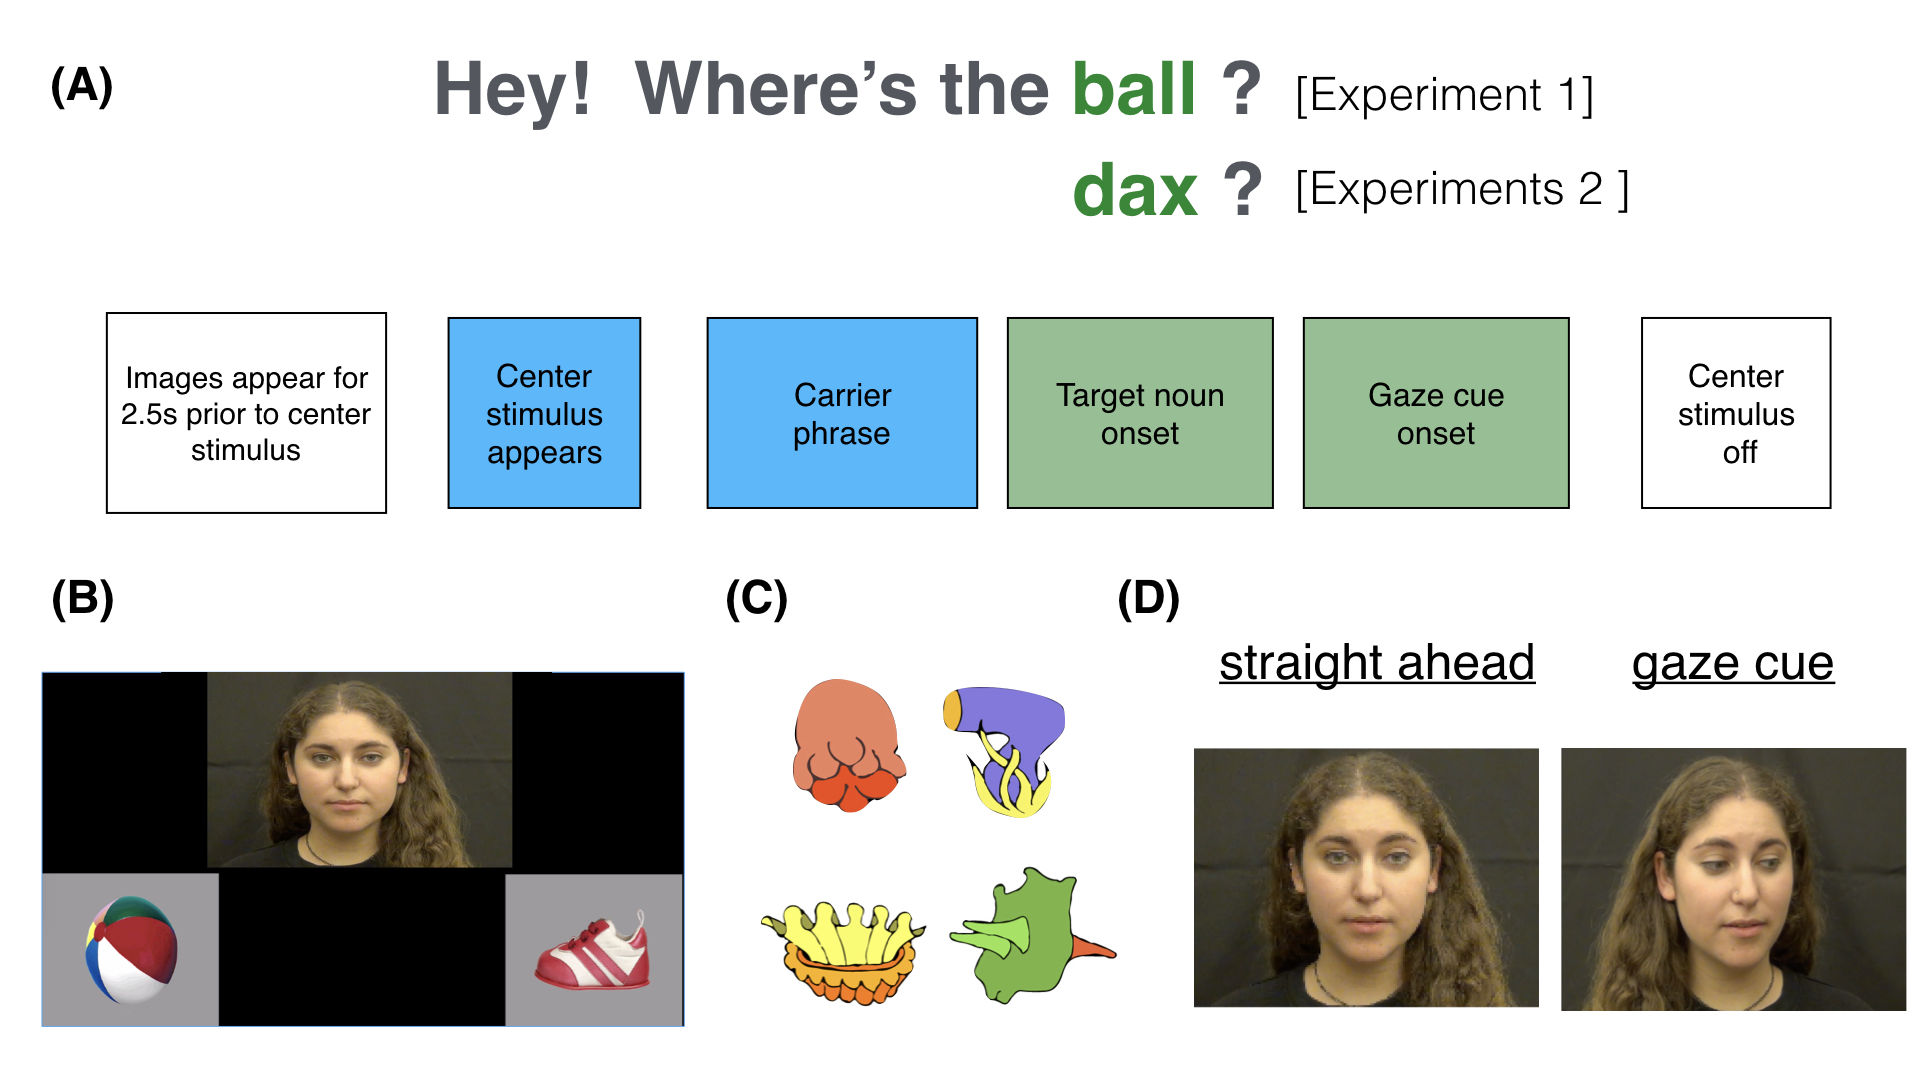
\includegraphics[width=0.9\linewidth]{/Users/kylemacdonald/Documents/Projects/SPEED-ACC-NOVEL/writing/figures/plots/gaze_stimuli} 

}

\caption{Stimuli for Experiments 1 and 3. Panel A shows the timecourse of the linguistic stimuli for a single trial. Panel B shows the layout of the fixation locations for all tasks: the center stimulus, the target, and the distracter. Panel C shows a sample of the images used as novel objects in Experiment 3. Panel D shows the social gaze manipulation.}\label{fig:gaze-stimuli}
\end{figure}

Participants viewed the task on a screen while their gaze was tracked
using an SMI RED corneal-reflection eye-tracker mounted on an LCD
monitor, sampling at 30 Hz. The eye-tracker was first calibrated for
each participant using a 6-point calibration. On each trial,
participants saw two images of familiar objects on the screen for two
seconds before the center stimulus appeared. Next, they processed the
target sentence -- which consisted of a carrier phrase, a target noun,
and a question -- followed by two seconds without language to allow for
a response. Both children and adults saw 32 trials (16 gaze trials; 16
no-gaze trials) with several filler trials interspersed to maintain
interest. The gaze manipulation was presented in a blocked design with
the order of block counterbalanced across participants.

\subsection{Results and Discussion}\label{results-and-discussion}

\emph{Timecourse looking.} We first analyzed how the presence of gaze
influenced listeners' distribution of attention across the three
fixation locations while processing familair words. At target-noun
onset, listeners tended to look more at the speaker than the objects. As
the target noun unfolded, the mean proportion looking to the center
decreased as participants shifted their gaze to the images. Proportion
looking to the target increased sooner and reached a higher asymptote
compared to proportion looking to the distracter for both gaze
conditions with adults spending more time looking at the target compared
to children. After looking to the named referent, listeners tended to
shift their gaze back to the speaker's face.

\begin{figure}[!t]

{\centering 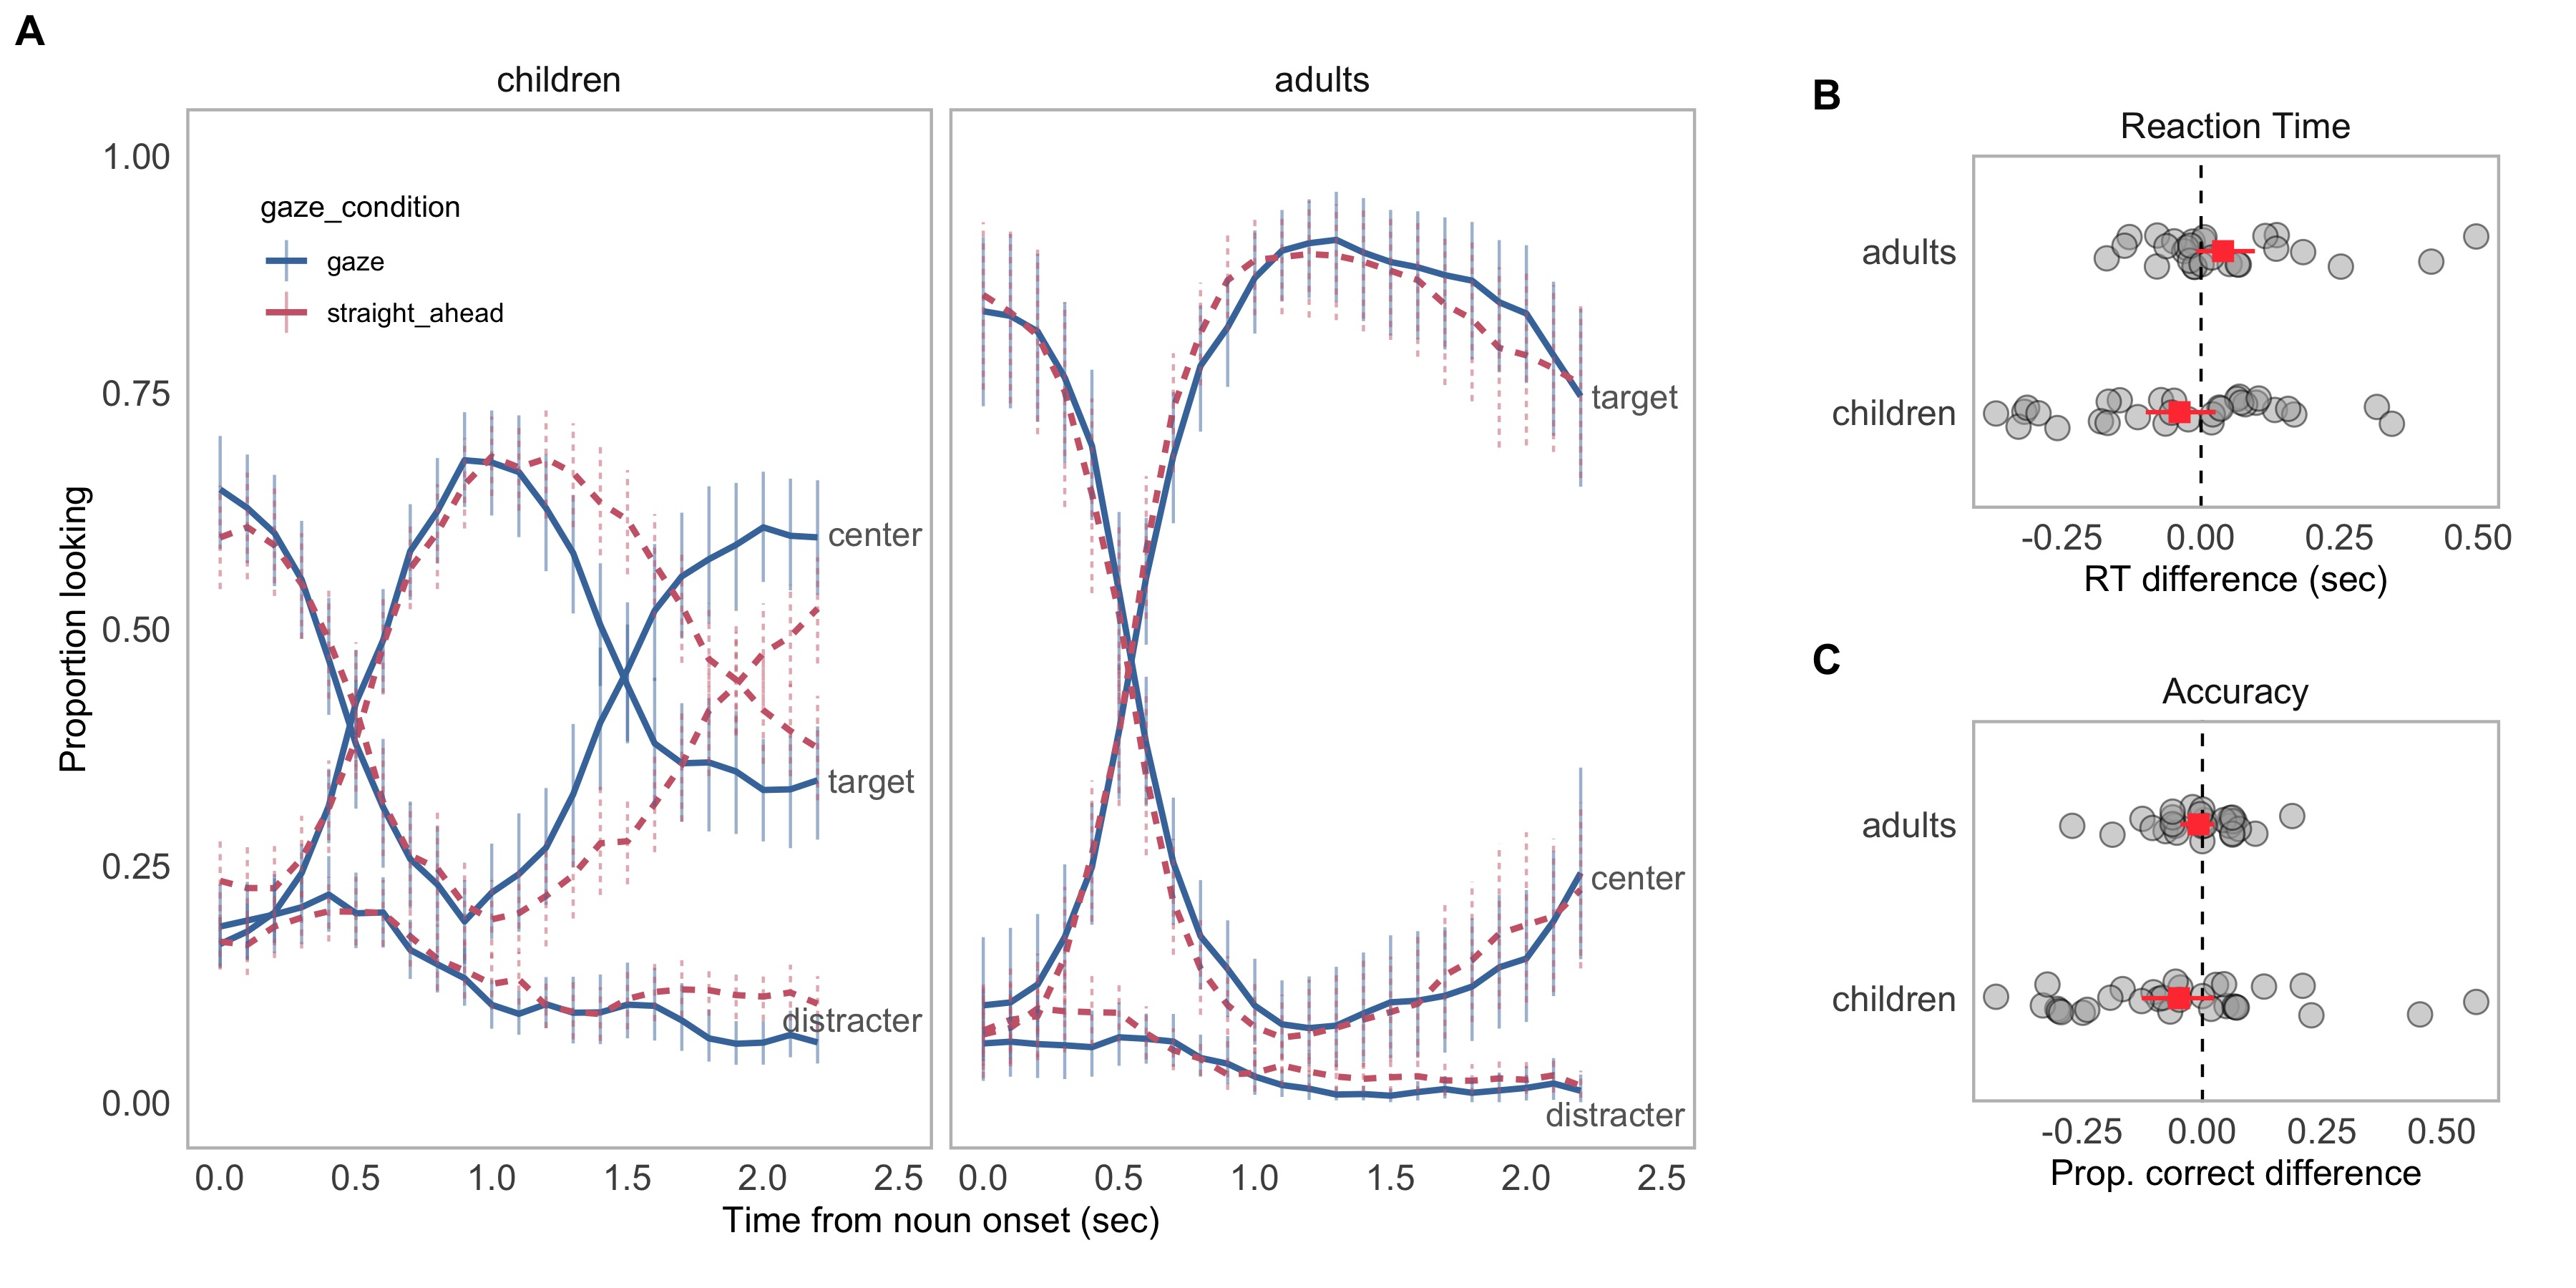
\includegraphics[width=0.95\linewidth]{/Users/kylemacdonald/Documents/Projects/SPEED-ACC-NOVEL/writing/figures/plots/speed_acc_fam_behav} 

}

\caption{Timecourse looking, first shift Reaction Time (RT), and Accuracy results for children in Experiment 1. Panel A shows the overall looking to the center, target, and distracter stimulus for each context. Panel B shows the distribution of pairwise contrasts between RTs in the gaze and no-gaze conditions. The square point represents the mean value for each measure. The vertical dashed line represents the null model of zero condition difference. The width each point represents the 95\% HDI. Panel C shows the same information but for participants' first shift accuracy.}\label{fig:speed-acc-gaze-results}
\end{figure}

We did not see evidence that the presence of a post-nominal gaze cue
changed how children or adults allocated attention early in the target
word. Children in the gaze condition, however, tended to shift their
attention back to the speaker earlier in the time course and spent more
time fixating on the speaker's face throughout the rest of the trial
(\(p < .001\); nonparametric cluster-based permutation analysis). Next,
we ask how these different processing contexts changed the timing and
accuracy of children's initial decisions to shift away from the center
stimulus.

\emph{First shift RT and Accuracy.} To quantify differences across the
groups, we fit a Bayesian linear mixed-effects regression predicting
first shift RT as a function of gaze condition and age group:
\emph{Log(RT) \(\sim\) gaze condition + age group + (gaze\_condition +
item \textbar{} subject)}. Both children and adults generated similar
RTs in the gaze (children \(M_{rt}\) = 563.16 ms, adults \(M_{rt}\) =
652.40 ms) and no-gaze (children \(M_{rt}\) = 575.76 ms, adults
\(M_{rt}\) = 608.31 ms) conditions, with the null value of zero
condition differences falling within the 95\% credible interval
(\(\beta\) = -0.01, 95\% HDI {[}-0.09, 0.07{]}). Next, we fit the same
model to estimate first shift accuracy. Adults generated more accurate
gaze shifts (\(M\) = 0.90) compared to children (\(M\) = 0.64) with the
null value falling within the 95\% HDI (\(\beta_{age}\) = -1.75, 95\%
HDI {[}-2.19, -1.32{]}). Similar to the RT analysis, we did not find
strong evidence of a difference in performance across the gaze
conditions (\(\beta\) = 0.11, 95\% HDI {[}-0.19, 0.41{]}).

Taken together, the time course and first shift analyses suggest that
hearing a familiar noun was sufficient for both adults and children to
drive visual attention away from the speaker to seek the named referent.
Morever, neither age group showed evidence of delaying their gaze shifts
to fixate on the speaker's face and gather a social cue to reference
that could have provided additional disambiguating information. The
presence of gaze, however, did affect children's looking behavior later
in the trial such that they were more likely to allocate attention to
the speaker when she had gazed at the named object. While we did not
predict these results, it is interesting that children's gaze dynamics
did not change when processing highly familiar words in the presence of
a social cue. This behavior seems reasonable if eye movements in
response to familiar language are highly-practiced visual routines that
do not allocate fixations to less-relevant locations. Moreover, if
children developed an expectation that their goal was to find named
objects quickly, then fixating the speaker becomes less goal-relevant.

In our previous work, we found that both children and adults fixate
longer on a speaker when language is more difficult to process because
of background noise (MacDonald, Marchman, Fernald, \& Frank, 2018). We
explained this result as an adaptation to the informational demands of
listeners' environment such that they were seeking additional visual
information to support language comprehension. The results of Experiment
1 can constrain our information seeking explanation by showing that
children do not always gather more visual information; instead, they
respond to the uncertainty in the input and adapt gaze to seek
information when uncertainty is higher. This raises an interesting
question: Would children's information seeking adapt when they do not
know the word-object mappings? That is, when the learner is surrounded
by novel objects, the value of seeking visual information from a social
partner should increase since this action could provide highly-relevant
information for decreasing referential uncertainty -- a point that has
long been emphasized by social-pragmatic theories of language
acquisition (P. Bloom, 2002; Clark, 2009; Hollich et al., 2000).
Experiments 2 and 3 explore this interesting case and ask whether
learners would adapt their gaze patterns to seek supprortive visual
information from social partners in the context of mapping novel words
to their referents.

\section{Experiment 2}\label{experiment-2}

Because children hear language in environments with multiple possible
referents, learning the meaning of even the simplest word requires
reducing this uncertainty. A cross-situational statistical learner can
aggregate across ambiguous naming events to learn stable word meanings.
But for this aggregation process to work, learners must allocate their
limited attention and memory resources to the relevant statistics in the
world -- how do they select what information to store?

In prior work (discussed in Chapter 4), we found that the presence of a
gaze cue shifted adults away from storing multiple word-object links and
towards tracking a single hypothesis. Those experiments, however, relied
on an offline measurement of word learning (a button press on test
trials) and an indirect measure of attention during learning (self-paced
decisions about how long to inspect the visual scene during learning
trials). We begain to address these limitations in a pilot study where
we adapted the social cross-situational learning paradigm to use
eye-tracking methods. Moving to an eye-tracking procedure allowed us to
ask (1) how does the presence of gaze alter the distribution of visual
attention during labeling? and (2) does the presence of a gaze cue
change the strength of learners' inferences about word-object links?

\subsection{Methods}\label{methods-1}

\subsubsection{Participants}\label{participants-1}

34 undergraduate students were recruited from the Stanford Psychology
One credit pool (17 F). Four participants were excluded during analysis
because the eye-tracker did not properly record their gaze coordinates.
The final sample included 30 participants.

\subsubsection{Materials}\label{materials-1}

The experiment featured sixteen pseudo-words recorded by an AT\&T
Natural VoicesTM speech synthesizer using the \enquote{Crystal}" voice
(a woman's voice with an American English accent), as well as 48 novel
objects represented by black-and-white drawings of fictional objects
from Kanwisher, Woods, Iacoboni, and Mazziotta (1997). Sixteen words
were used so that the experiment would be sufficiently long to make
within-subject comparisons across trials, and 48 objects were used so
that objects would not be repeated across trials. Six familiar objects
from the same set of drawings were used for the two practice trials,
accompanied by two familiar words using the same speech synthesizer.
Finally, the videos of the speaker's face were taken from from
MacDonald, Yurovsky, and Frank (2017).

\subsubsection{Procedure}\label{procedure-1}

We tracked adults' eye movements while they watched a series of
ambiguous word-learning events (16 novel words) organized into pairs of
exposure and test trials (32 trials total). All trials consisted of a
set of two novel objects and one novel word. Participants were randomly
assigned to either the Gaze condition in which a speaker looked at one
of the objects on exposure trials or the No-Gaze condition in which a
speaker looked straight on exposure trials. Every exposure trial was
followed by a test trial, where participants heard the same novel word
paired with a new set of two novel objects. One of the objects in the
set had appeared in the exposure trial (\enquote{target} object), while
the other object had not previously appeared in the experiment
(\enquote{distracter} object).

\begin{figure}[!t]

{\centering 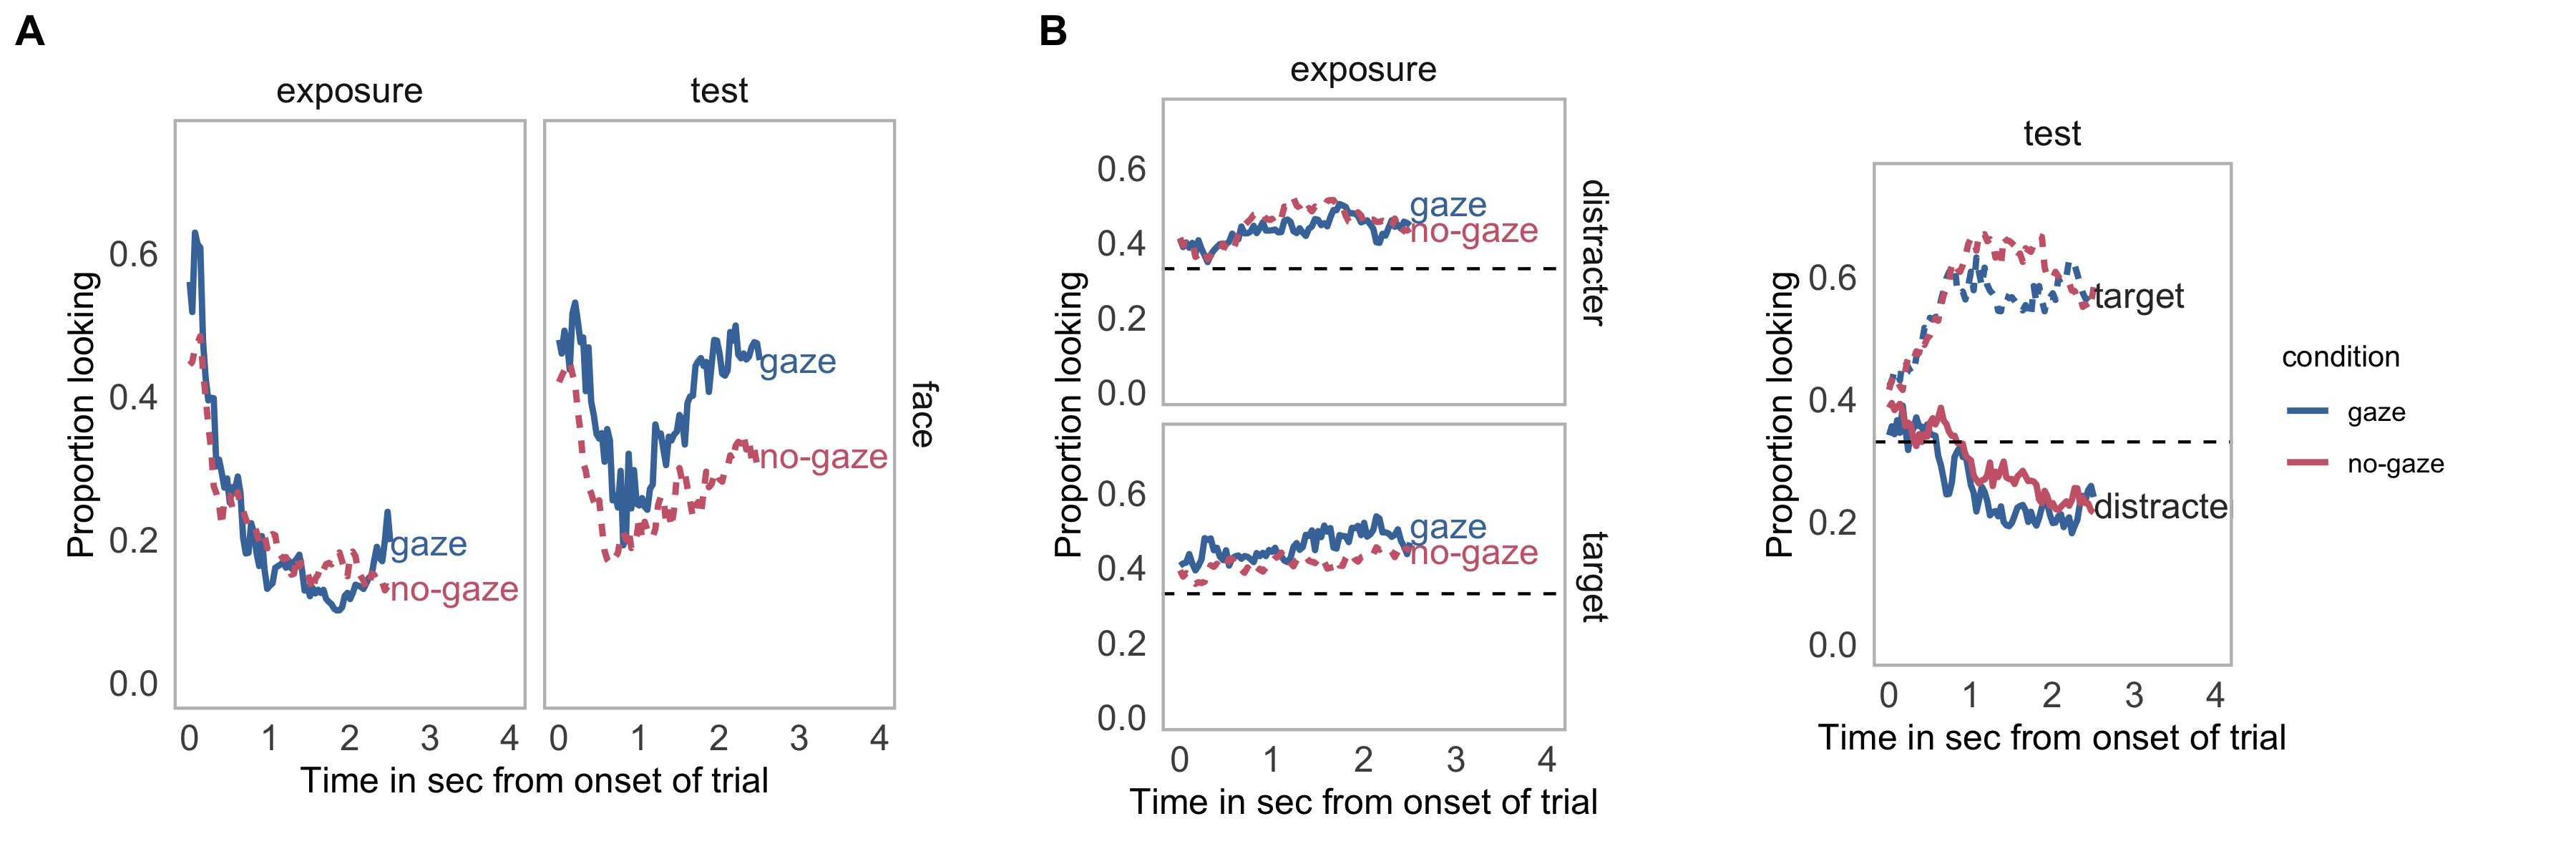
\includegraphics[width=1\linewidth]{/Users/kylemacdonald/Documents/Projects/SPEED-ACC-NOVEL/writing/figures/plots/gaze_xsit_tc} 

}

\caption{Overview of adults' looking to the three fixation targets (Face, Target, Distracter) over the course of the trial. Panel A shows proportion looking to the speaker's face for exposure and test trials. Color and linetype represent gaze condition. Panel B shows the same information but for proportion looking to the target and distracter images.}\label{fig:gaze-xsit-tc-plot}
\end{figure}

The side of the screen of the target object was counterbalanced
throughout the experiment. In the gaze condition, for half of the test
trials, the target object was the focus of the speaker's gaze during the
exposure trial, while the other half, the target object was the object
that had not been the focus of gaze during labeling.

\subsection{Results and Discussion}\label{results-and-discussion-1}

\emph{Timecourse looking.} The first question of interest was how did
the presence of a gaze cue change adults' distribution of attention
across the three fixation locations while processing language in
real-time? Figure~\ref{fig:gaze-xsit-tc-plot} presents an overview of
looking to each AOI for each processing context. This plot shows changes
in the mean proportion of trials on which participants fixated on the
speaker's face, the target image, or the distracter image at every 33-ms
interval of the stimulus sentence. At target-noun onset, adults tended
to look more at the speaker's face on both exposure and test trials. As
the target noun unfolded, the mean proportion looking to the center
decreased as participants shifted their gaze to the target or the
distracter images. On exposure trials tended to distribute their
attention relatively evenly across target and distracter images. On test
trials, proportion looking to the target increased sooner and reached a
higher asymptote compared to proportion looking to the distracter for
both condition, suggesting that adults were able to track the consistent
word-object links in both conditions.

There were several qualitative differences in looking behavior across
the different gaze conditions and trial types. First, adults spent more
time looking to a speaker's face when she provided a social gaze cue,
especially on test trials that were preceded by gaze (Panel A of Figure
XXX). Second, adults in the gaze condition looked slightly more to the
target image over the course of the trial. This behavior is reasonable
since half of the trials, the speaker's gaze was focused on the target
image that would appear on the subsequent test trial. Third, on test
trials, adults looked more to the images in the no-gaze context. This
led to a higher proportion of looking to the target, but also a higher
proportion of looking to the distracter images (Panel B of Figure XXX).

Together, these looking patterns provide preliminary evidence that the
presence of a gaze cue caused adults to spend more time gathering visual
information from the speaker's face. Next, we ask how the social gaze
cue modulated learning, which we operationalized as the relationship
between looking behavior on exposure and test trials.

\begin{figure}[!t]

{\centering 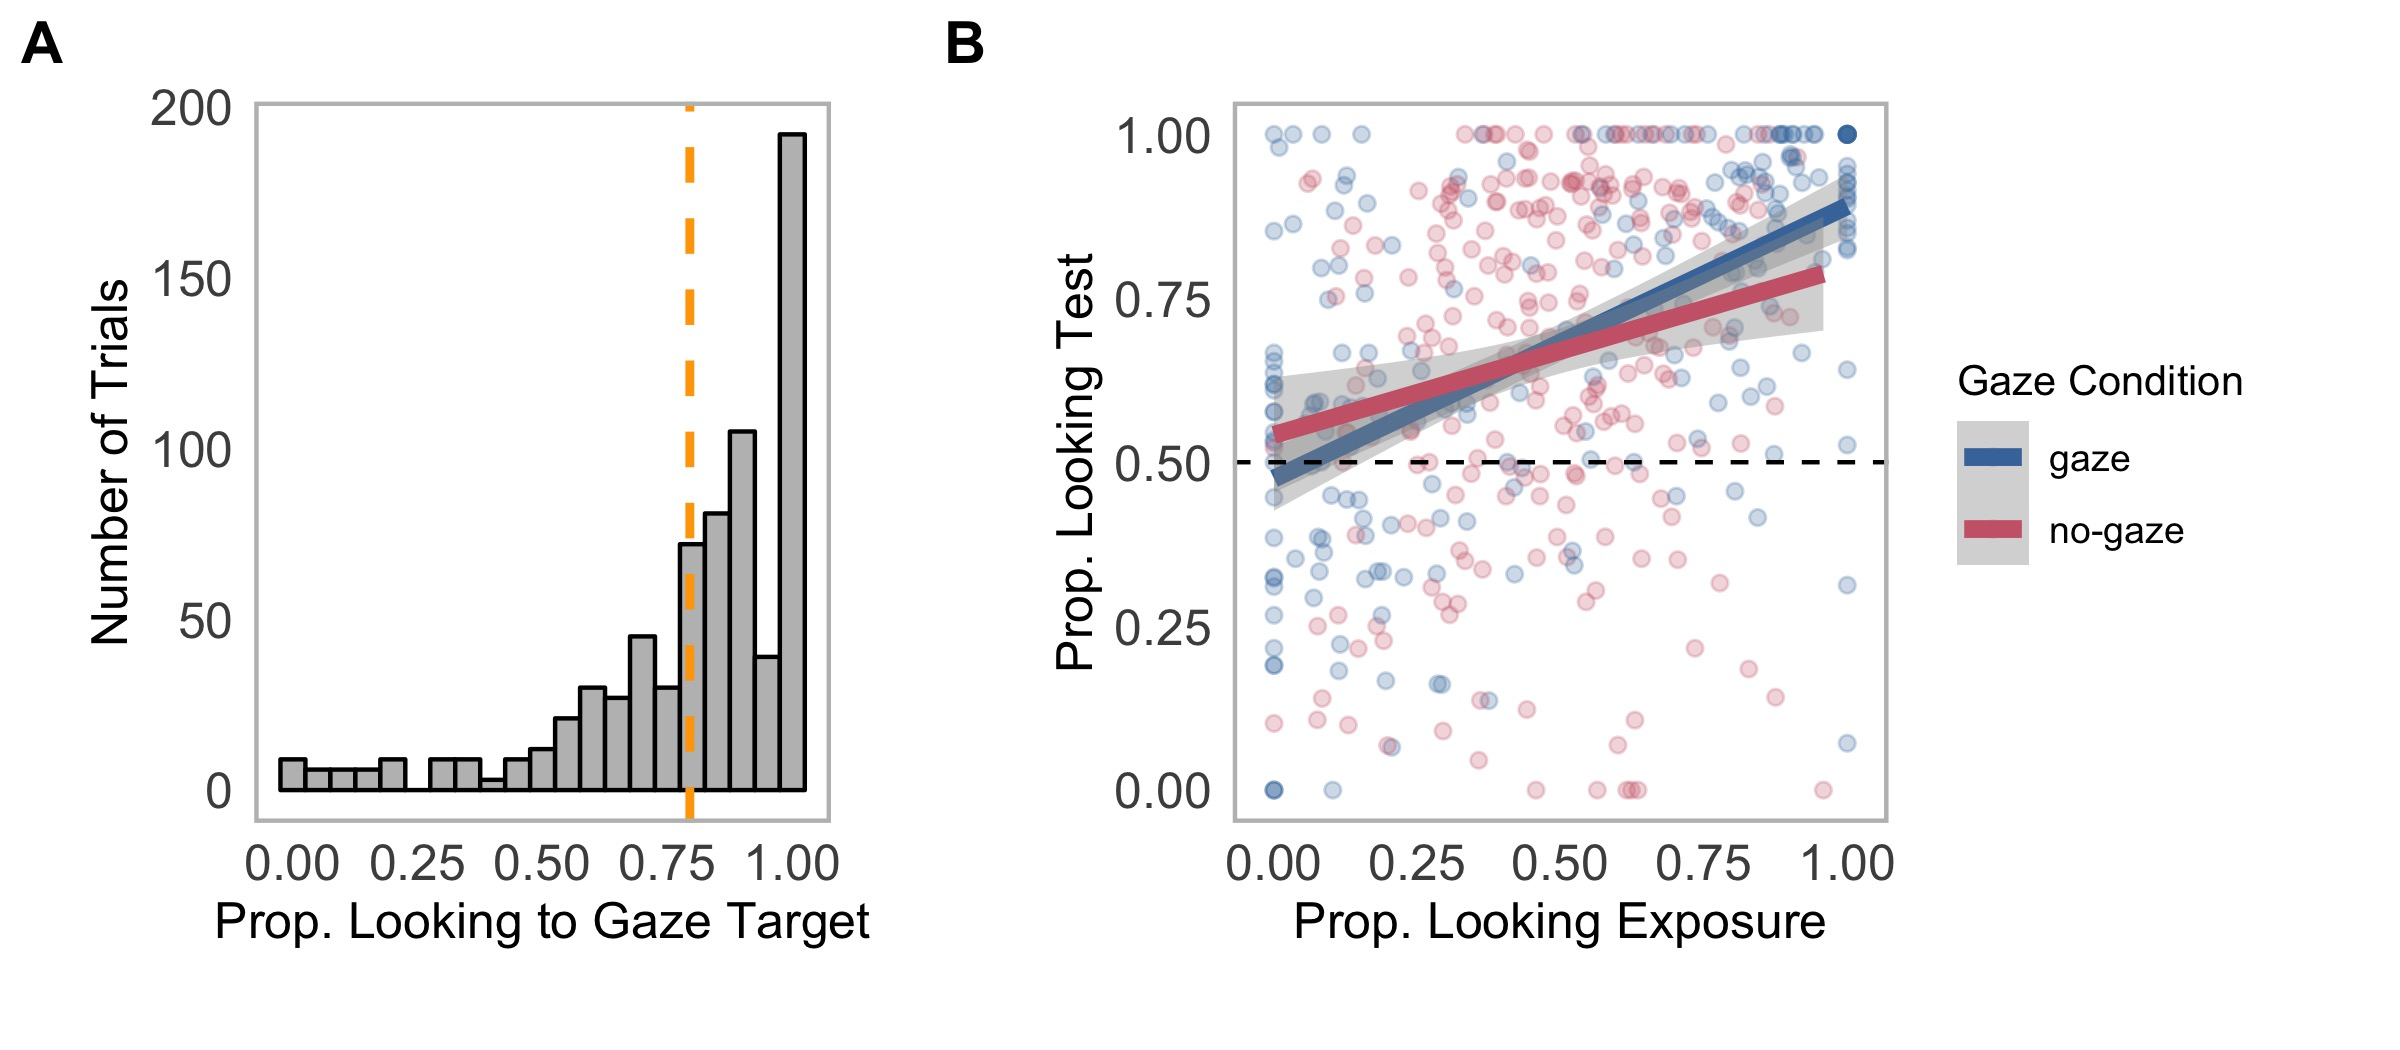
\includegraphics[width=0.9\linewidth]{/Users/kylemacdonald/Documents/Projects/SPEED-ACC-NOVEL/writing/figures/plots/gaze_xsit_prop_looking} 

}

\caption{Panel A shows participants’ tendency to look at the object that was the target of the speaker’s gaze on exposure trials. The vertical, dashed line represents the mean proportion of time looking to the gaze target across all trials. Panel B shows the relationship between adults' looking behavior on exposure and test trials for the gaze and no-gaze conditions.}\label{fig:gaze-xsit-prop-looking-plot}
\end{figure}

\emph{Relationship between performance on exposure and test trials.}
When the speaker generated a social cue during labeling, adults reliably
followed that cue and tended to focus their attention on a single object
(Figure XXXA). In contrast, people in the No-gaze condition tended to
distribute their attention more broadly across the two objects. For
adults in both gaze contexts, more time spent attending to the target
object on exposure trials led higher proportion looking to the target,
i.e., better recall, at test (\(\beta_{exposure}\) = 0.43, 95\% HDI
{[}0.36, 0.50{]}). Critically, there was an interaction between the gaze
condition and the relationship between attention on exposure and test:
When eye gaze cued visual attention, adults showed stronger memory for
the word-object link (\(\beta_{int}\) = -0.19, 95\% HDI {[}-0.33,
-0.05{]}). This result provides evidence that social information does
not only modulate people's in-the-moment decisions about how to allocate
their visual attention; instead, the social cue changed the strength of
the memory for word-object links that are stored during
cross-situational word learning.

\subsubsection{Limitations}\label{limitations}

There were several key limitations of our pilot study. First, we chose
to start the liguistic stimulus as soon as the images and the speaker
appeared on the screen (i.e., at trial onset). This made it difficult to
analyze the timing and accuracy of first shifts decisions away from the
speaker and to the objects. Second, this trial structure did not allow
us to measure decisions about visual fixation that occur before the
start of language comprehension while learners are first gathering
information about the visual world. Finally, the linguistic stimuli
consisted of sixteen pseudowords recorded by a speech synthesizer and
presented in isolation, thus removing any sentential context. Presenting
isolated words is unlikely to work with younger age groups and does not
allow us to separate decisions about fixations made during language
processing more broadly from decisions that occur after the onset of the
target noun -- a critical distinction for our modeling of the underlying
decision-making process. Experiment 3 was designed to address these
limitations and to ask how learners' information seeking from social
partners changes as a function of increased exposure to word-object
mappings (i.e., disambiguating statistical information).

\section{Experiment 3}\label{experiment-3}

Experiment 3 was designed to ask how social information modulates
learners' real-time visual information selection as they accumulate
knowledge about novel word-object links.\footnote{See
  \url{https://osf.io/nfz85/} for a pre-registration of the analysis
  plan and predictions.} We also set out to address the limitations of
Experiment 2 discussed above. There were two key modifications. First,
we modified the cross-situational learning paradigm to include more than
two exposures to a novel word-object link. This allowed us to measure
changes in learners' integration of social and statistical information
over a longer timescale. Second, we changed the linguistic stimuli to
parallel the design of Experiment 1 such that the novel words occurred
within a target sentence. This allowed us to leverage the analytic
techniques developed for analyzing participants' initial gaze shifts in
Experiment 1 to ask how decisions about visual information gathering
from social partners changed as a function of repeated exposure to
statistical information about word-object mappings.

\noindent
We aimed to answer the following specific research questions:

\begin{enumerate}
\def\labelenumi{\arabic{enumi}.}
\tightlist
\item
  How do decisions about where to allocate visual attention (speakers
  vs.~objects) change as a function of learning a new word?
\item
  How does the presence of a social cue to reference (eye gaze) change
  the dynamics of children's gaze patterns during object labeling?
\item
  What is the relationship between chidren's gaze patterns during object
  labeling and their memory of new words?
\end{enumerate}

To answer these questions, we compared the timing and accuracy of eye
movements during a real-time cross-situational learning task where
participants process sentences that contain a novel word (e.g.,
\enquote{Where's the \emph{dax}?}) while looking at a simplified visual
world with 3 fixation targets (a video of a speaker and two images of
unfamiliar objects).

\subsection{Predictions}\label{predictions}

We had three key behavioral predictions. First, for all conditions,
participants' distribution of attention to speakers compared to objects
will shift over the course of learning. Early in the task, participants
will allocate more fixations to a speaker to prioritize gathering visual
information that disambiguates reference. After experiencing multiple
exposures to a word-object pairing, participants will generate faster
saccades, showing signatures of comprehension of the incoming speech. We
further predict that later in learning blocks, participants will
allocate more fixations to the objects, showing looking behaviors that
support learning long-term associations between words and objects.

Second, the presence of a gaze cue will change participants' decisions
about visual fixation. We hypothesize that a post-nominal gaze cue
increases the value of fixating on a speaker. This manipulation will
cause participants to allocate more fixations to the speaker when gaze
is present, leading to slower first shift reaction times and higher
proportion looking, especially earlier in learning (i.e., lower trial
numbers within each block of exposure trials to a novel word-object
pairing). This prediction will be operationalized as a main effect of
Gaze condition on RT, and a trial number by Gaze condition interaction
such that the decrease in RT will be greater on exposure trials in the
Gaze condition.

Third, the Gaze condition should lead to stronger inferences about the
correct word-object mapping, resulting in faster learning that we
operationalize as more accurate first shifts, faster RTs, and a higher
proportion looking to the target vs.~the distractor object on test
trials as compared to learning words without a gaze cue across both
exposure and test trials.

\subsection{Methods}\label{methods-2}

\subsubsection{Participants}\label{participants-2}

Participants were native, monolingual English-learning children (\(n=\)
54; 30 F) and adults (\(n=\) 10; 5 F). All participants had no reported
history of developmental or language delay and normal vision. 6 adults
were run but not included in the analysis because they were not native
speakers of English. XXX participants were run but not included in
analysis because either the eye tracker falied to calibrate (XXX
children, XXX adults) or the participant did not complete the task (XXX
children).

\subsubsection{Materials}\label{materials-2}

\emph{Linguistic stimuli.} The video/audio stimuli were recorded in a
sound-proof room and featured two female speakers who used natural
child-directed speech and said one of two phrases: \enquote{Hey! Can you
find the (novel word)} or ``Look! Where's the (novel word). The target
words were four pseudo-words: bosa, modi, toma, and pifo. The novel
words varied in length (shortest = XXX ms, longest = XXX ms) with an
average length of XXX ms.

\emph{Gaze manipulation}. To create the stimuli in the gaze condition,
the speaker waited until she finished producing the novel word before
turning her head to gaze at the bottom right corner of the frame. After
looking at the named object, she then returned her gaze to the center of
the frame. We chose to allow the length of the gaze cue to vary to keep
the stimuli naturalistic. The average length of gaze was 2.12 seconds
with a range from 1.78 to 3.07 seconds.

\emph{Visual stimuli.} The image set consisted of 28 colorful digitized
pictures of objects that were selected such that children were unlikely
to already have a label associated with them. The side of the target
picture was counterbalanced across trials.

\subsubsection{Procedure}\label{procedure-2}

Participants viewed the task on a screen while their gaze was tracked
using an SMI RED corneal-reflection eye-tracker mounted on an LCD
monitor, sampling at 30 Hz. The eye-tracker was first calibrated for
each participant using a 6-point calibration. Then, participants watched
a series of ambiguous word learning events organized into pairs of one
exposure and one test trial. On each trial, participants saw of a set of
two unfamiliar objects and heard one novel word.

Each word was learned in a block of four exposure-test pairs for a total
of eight trials for each novel word. Critically, on each trial within a
word block, one of the objects in the set had appeared on the previous
trials (target object), while the other object was a randomly generated
novel object not previously shown in the experiment (distracter object).
Both children and adults saw 32 trials (16 gaze trials; 16 no-gaze
trials) with several filler trials interspersed to maintain interest.
The gaze manipulation was presented in a blocked design with the order
of block counterbalanced across participants.

\subsection{Results and Discussion}\label{results-and-discussion-2}

\subsubsection{Timecourse looking}\label{timecourse-looking}

\begin{figure}[!t]

{\centering 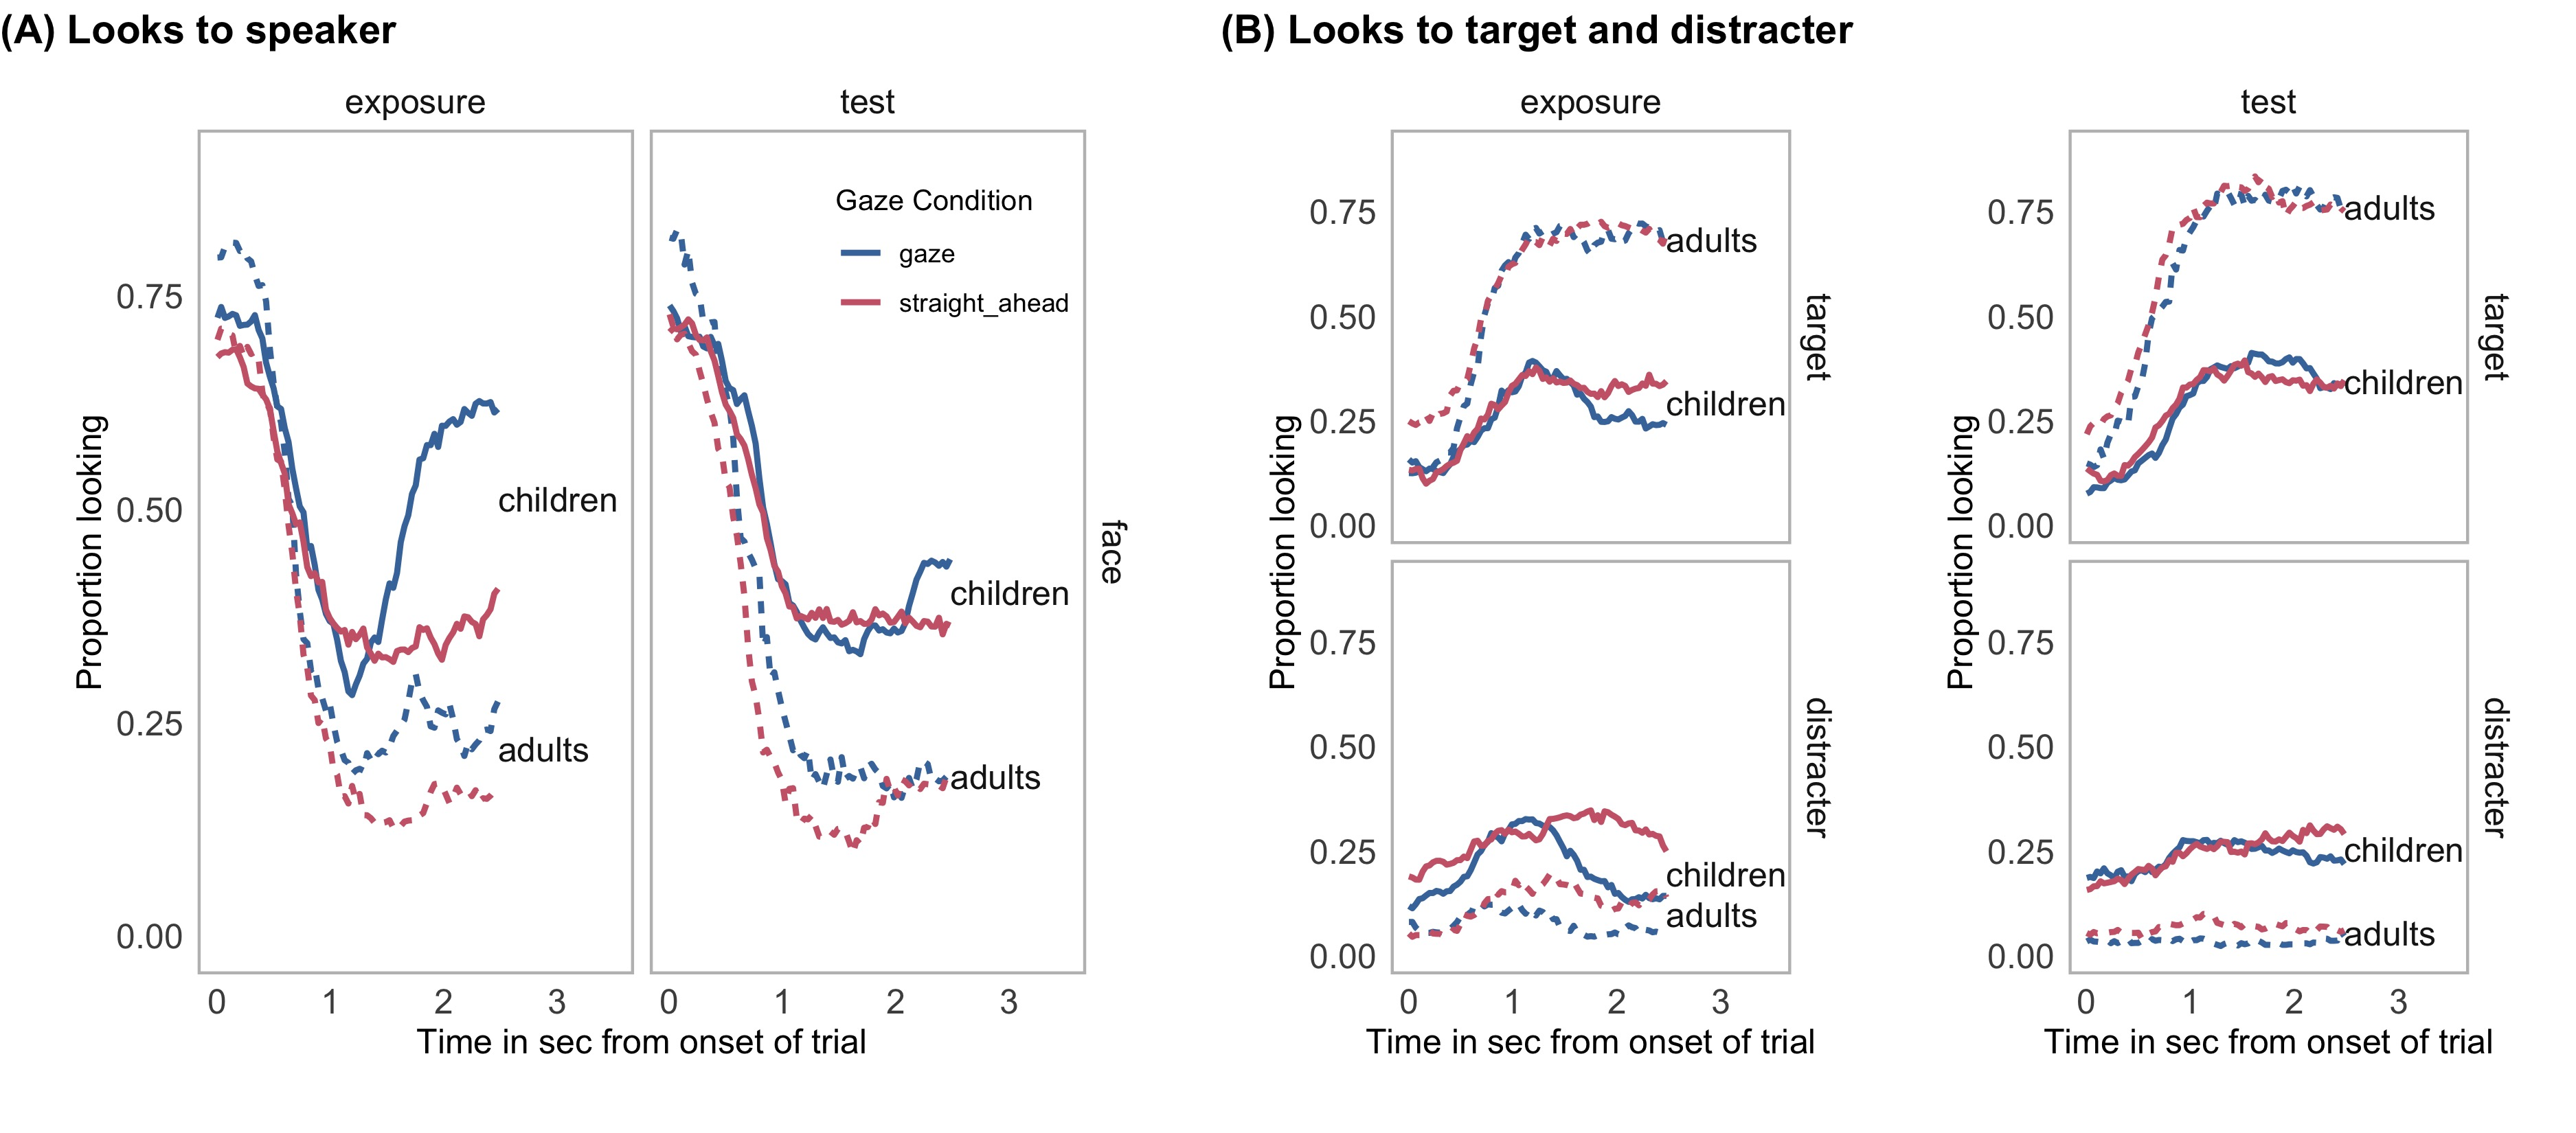
\includegraphics[width=1\linewidth]{/Users/kylemacdonald/Documents/Projects/SPEED-ACC-NOVEL/writing/figures/plots/speed_acc_novel_tc} 

}

\caption{Overview of children and adults' looking to the three fixation targets (Speaker, Target, Distracter) over the course of exposure and test trials. Panel A shows proportion looking to the speaker's face with color indicating gaze condition and linetype indicating age group. Panel B shows the same information but for proportion looking to the target and distracter images.}\label{fig:san-tc-plot}
\end{figure}

\emph{Looking to the speaker.} How did the presence of a gaze cue change
learners' decisions to fixate on the speaker? In Figure XXXA, we see
that both children and adults tended to start looking at the speaker at
noun onset and shifted their gaze away as the noun unfolded, with adults
doing so sooner compared to children. On Exposure trials when there was
a gaze cue, both adults and children tended to look more to the face at
noun onset as indicated by the higher intercept of the blue curves.
Moreover, around one second after noun onset, listeners tended to shift
their attention back to the speaker's face more often and especially so
for children. On Test trials that were preceded by an Exposure trial
with a gaze cue, children and adults tended to look more to the speaker
even though there was no gaze cue present. This pattern of results
provides suggestive evidence that the presence of gaze modulated
learners' expectations of dismabiguating information from the speaker.

\emph{Looking to the target and distracter.} Next, we asked how learners
divided attention between the target and distracter objects. On Exposure
trials, looking to both objects increased over the course of the trial
but more so for looks to the named object as indicated by the higher
asymptote of the target looking curves. Adults spent more time looking
to the target and less time looking to the distracter as compared to
children. For both children and adults, there was evidence that
proportion looking to the target was higher on Exposure trials in the
gaze condintion. There was a developmental difference, however, such
that higher proportion looking to the target generalized to Test trials
for adults but not for children who showed less robust learning of the
word-object links and similar performance across the gaze conditions.
The strongest effect of gaze was on the tendency to look at the
distracter object, with learners allocating fewer fixations to the
distracter when they could use a disambiguating gaze cue on Exposure
trials and even on Test trials that were preceded by Exposure trials
with a gaze cue.

\subsubsection{Proportion looking}\label{proportion-looking}

\emph{Learning effects.} Our primary question of interest was how
exposure to multiple co-occurrences of word-object pairs would change
learners' distribution of attention between the speaker and objects.
Figure XXX shows proportion looking to the speaker (XXXA) and the target
and distracter objects (XXXB) as a function of trial number within a
word learning block. Both children and adults were more likely to fixate
on the speaker when she provided a gaze cue (\(\beta_{gaze}\) = 0.09,
95\% HDI {[}0.17, 0.01{]}). Moreover, there was a developmental
difference such that children, but not adults, were more likely to
increase their fixations to the speaker over the course of the learning
block (\(\beta_{gaze:tr.num}\) = -0.07, 95\% HDI {[}-0.10, -0.04{]}).

\begin{figure}[!t]

{\centering 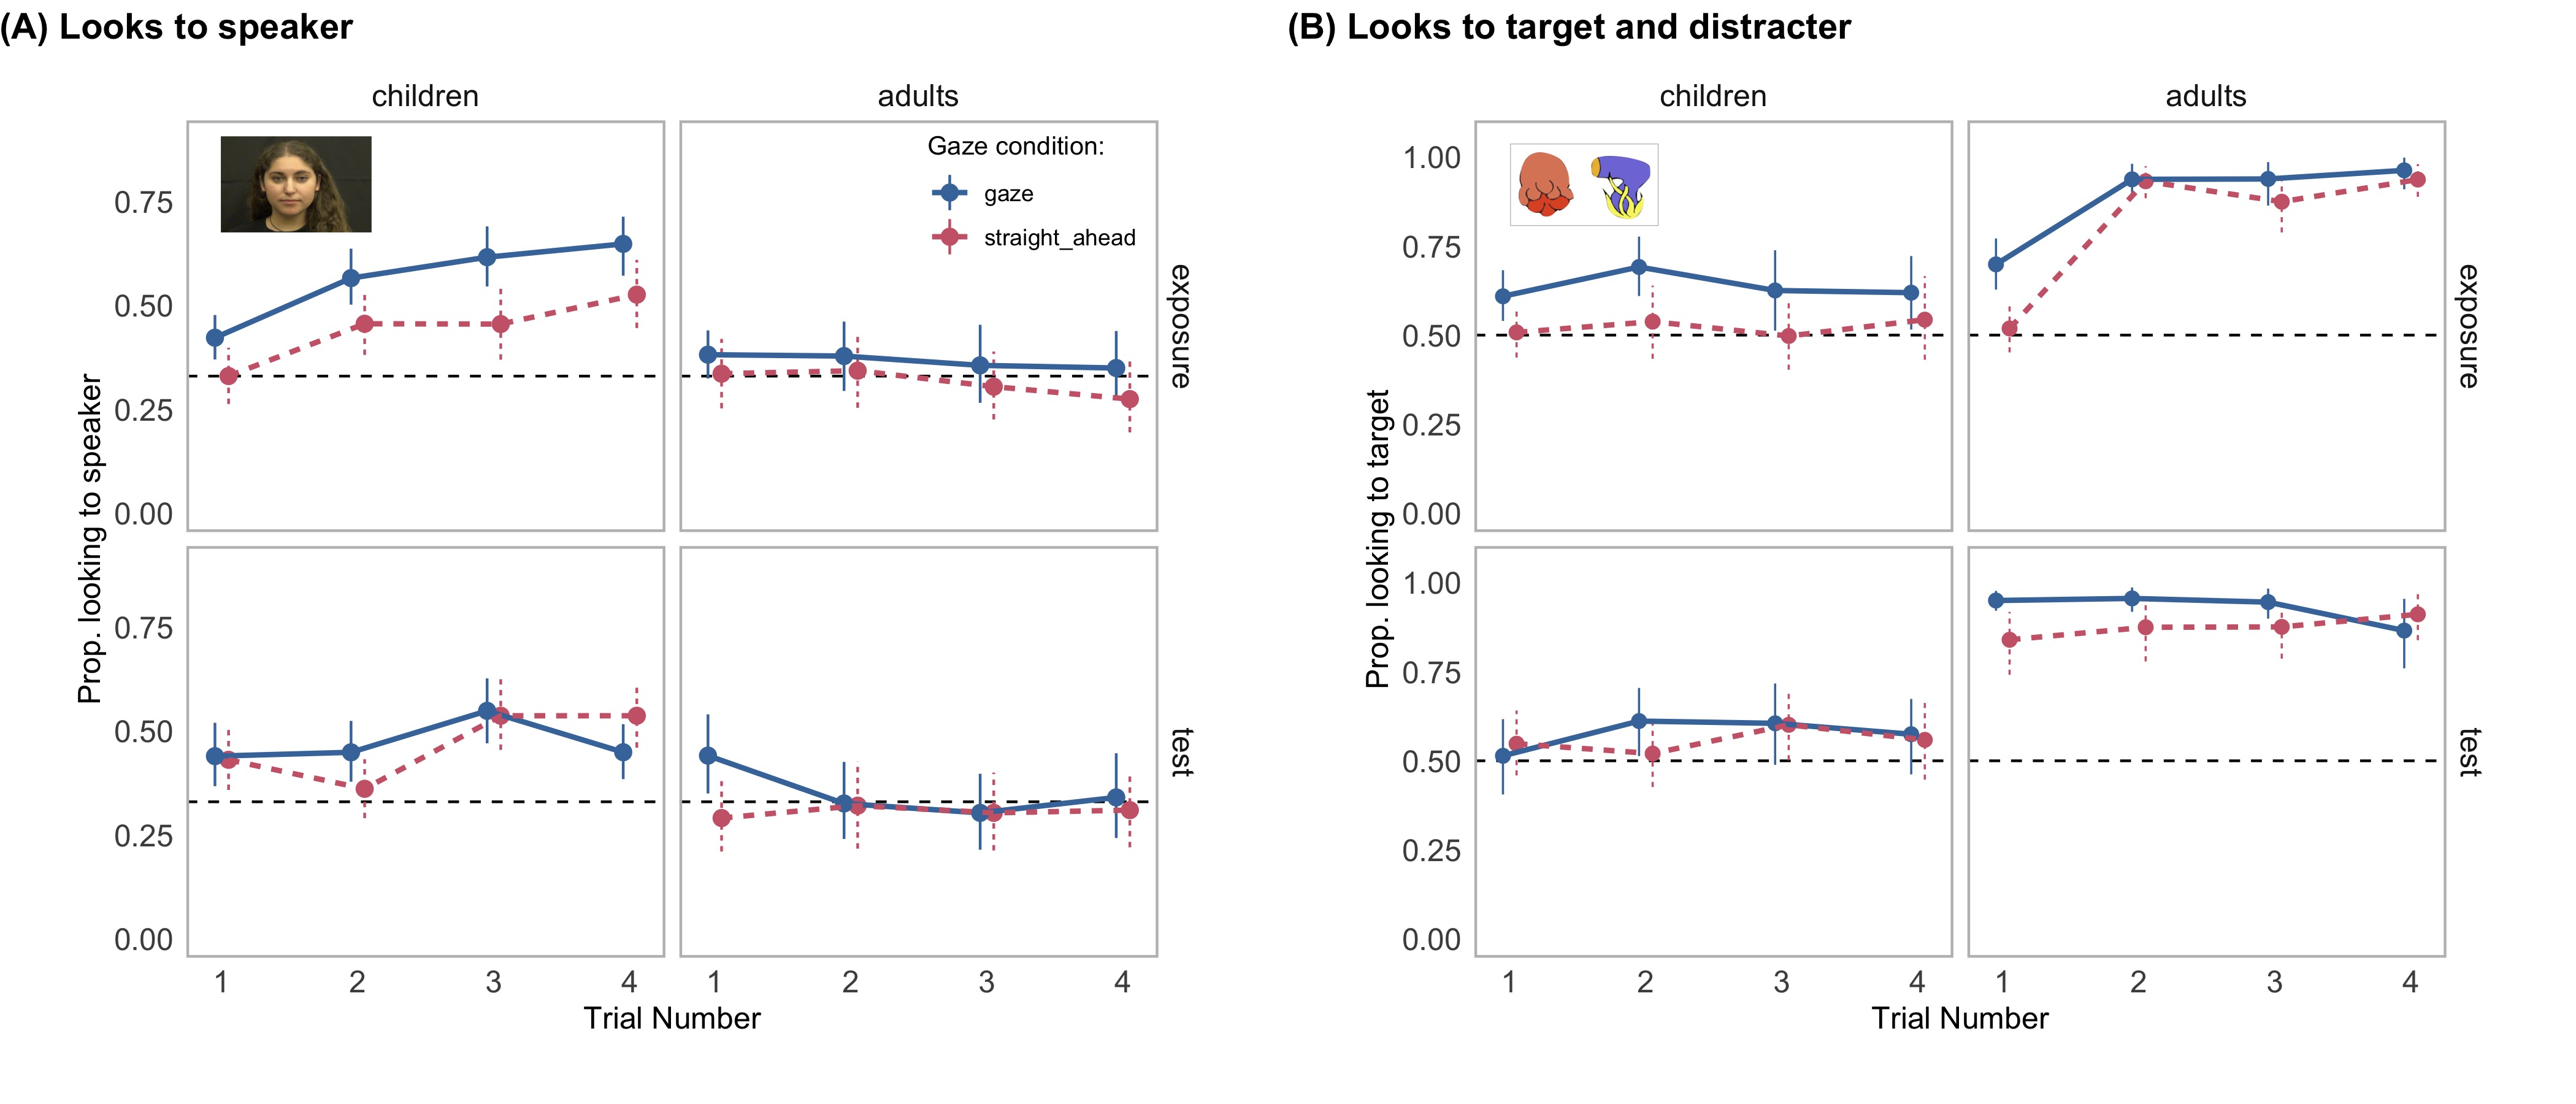
\includegraphics[width=1\linewidth]{/Users/kylemacdonald/Documents/Projects/SPEED-ACC-NOVEL/writing/figures/plots/speed_acc_novel_proplook} 

}

\caption{Panel A shows participants’ tendency to look at the target object on exposure and test trials as a function of the trial number within a learning block. The horizontal, dashed line represents the tendency to distribute attention equally across the two images. Color indicates gaze condition and error bars represent 95\% credible intervals. Panel B shows the same information but collapsed across trial to highlight the effect of the gaze cue.}\label{fig:san-prop-looking-plot}
\end{figure}

Overall, looking to the target increased as learners were exposed to
more word-object pairings (\(\beta_{tr.num}\) = 0.08, 95\% HDI {[}0.05,
0.10{]}) and was higher when the novel word was accompanied by a gaze
cue (\(\beta_{gaze}\) = -0.18, 95\% HDI {[}-0.26, -0.10{]}). Visual
inspection of Figure XXX shows that, on the first Exposure trial, both
adults and children used the gaze cue to disambiguate reference,
fixating more on the target in the Gaze condition. For children, higher
target looking on Exposure trials with gaze remained relatively constant
across the learning block. In contrast, adults target looking reached
ceiling for both Gaze and No-gaze conditions by trial number two,
indicating that they had successfully used the co-occurrence information
across trials to map the novel word to its referent. We also saw
evidence that adults, but not children, looked more to the target object
on Test trials preceded by Exposure trials with a gaze cue earlier in
the course of learning, with adults tending to achieve the same level of
accuracy on Test trials in the absence of gaze at the end of the
learning block. We did not see evidence for an effect of the gaze
manipulation on children's looking behavior on Test trials.

\emph{Relationship between looking on exposure and test.} For both
children and adults, more time attending to the target object on
exposure trials led to a higher proportion of looking to the target on
test trials, especially for adults (\(\beta_{exposure:age}\) = 0.16,
95\% HDI {[}0.05, 0.27{]}) and as the number of word-object exposures
increased over the course a learning block (\(\beta_{exposure:tr.num}\)
= 0.06, 95\% HDI {[}0.01, 0.11{]}). There was some evidence that
learners in the No-gaze context spent less time looking to the target
image on Test trials later in the learning block
(\(\beta_{gaze:tr.num}\) = -0.02, 95\% HDI {[}-0.04, 0.00{]}). This
result dovetails with the findings from Experiment 2, providing evidence
that the presence of social information did more than change attention
on Exposure trials but instead modulated the relationship between
attention during learning and laater memory for the word-object links.

Overall, the time course and the proportion looking analyses suggest
that the presence of gaze changed how children and adults allocated
attention while processing novel words. In the context of unfamiliar
objects, children tended to fixate more on a speaker's face when she
provided a post-nominal social cue to reference, a difference in looking
behavior that increased as they were exposed to more word-object
co-ocurrences. This result stands in contrast to the parallel looking
behavior that we found in Experiment 1 when children were processing
highly familiar nouns. Morever, in the presence of a speaker who
provides a gaze cue, children and adults spent less time fixating on the
distracter image, thus modulating the strength of the possible
word-object connections that could have been created during the labeling
moment. However, these changes in gaze patterns did not generalize to
performance differences on Test trials for children in this task.
Finally, there evidence that the presence of a social cue to reference
modulated the link between attention on exposure trials and fixations at
test.

\subsubsection{First shift RT and
Accuracy}\label{first-shift-rt-and-accuracy}

\begin{figure}[!t]

{\centering 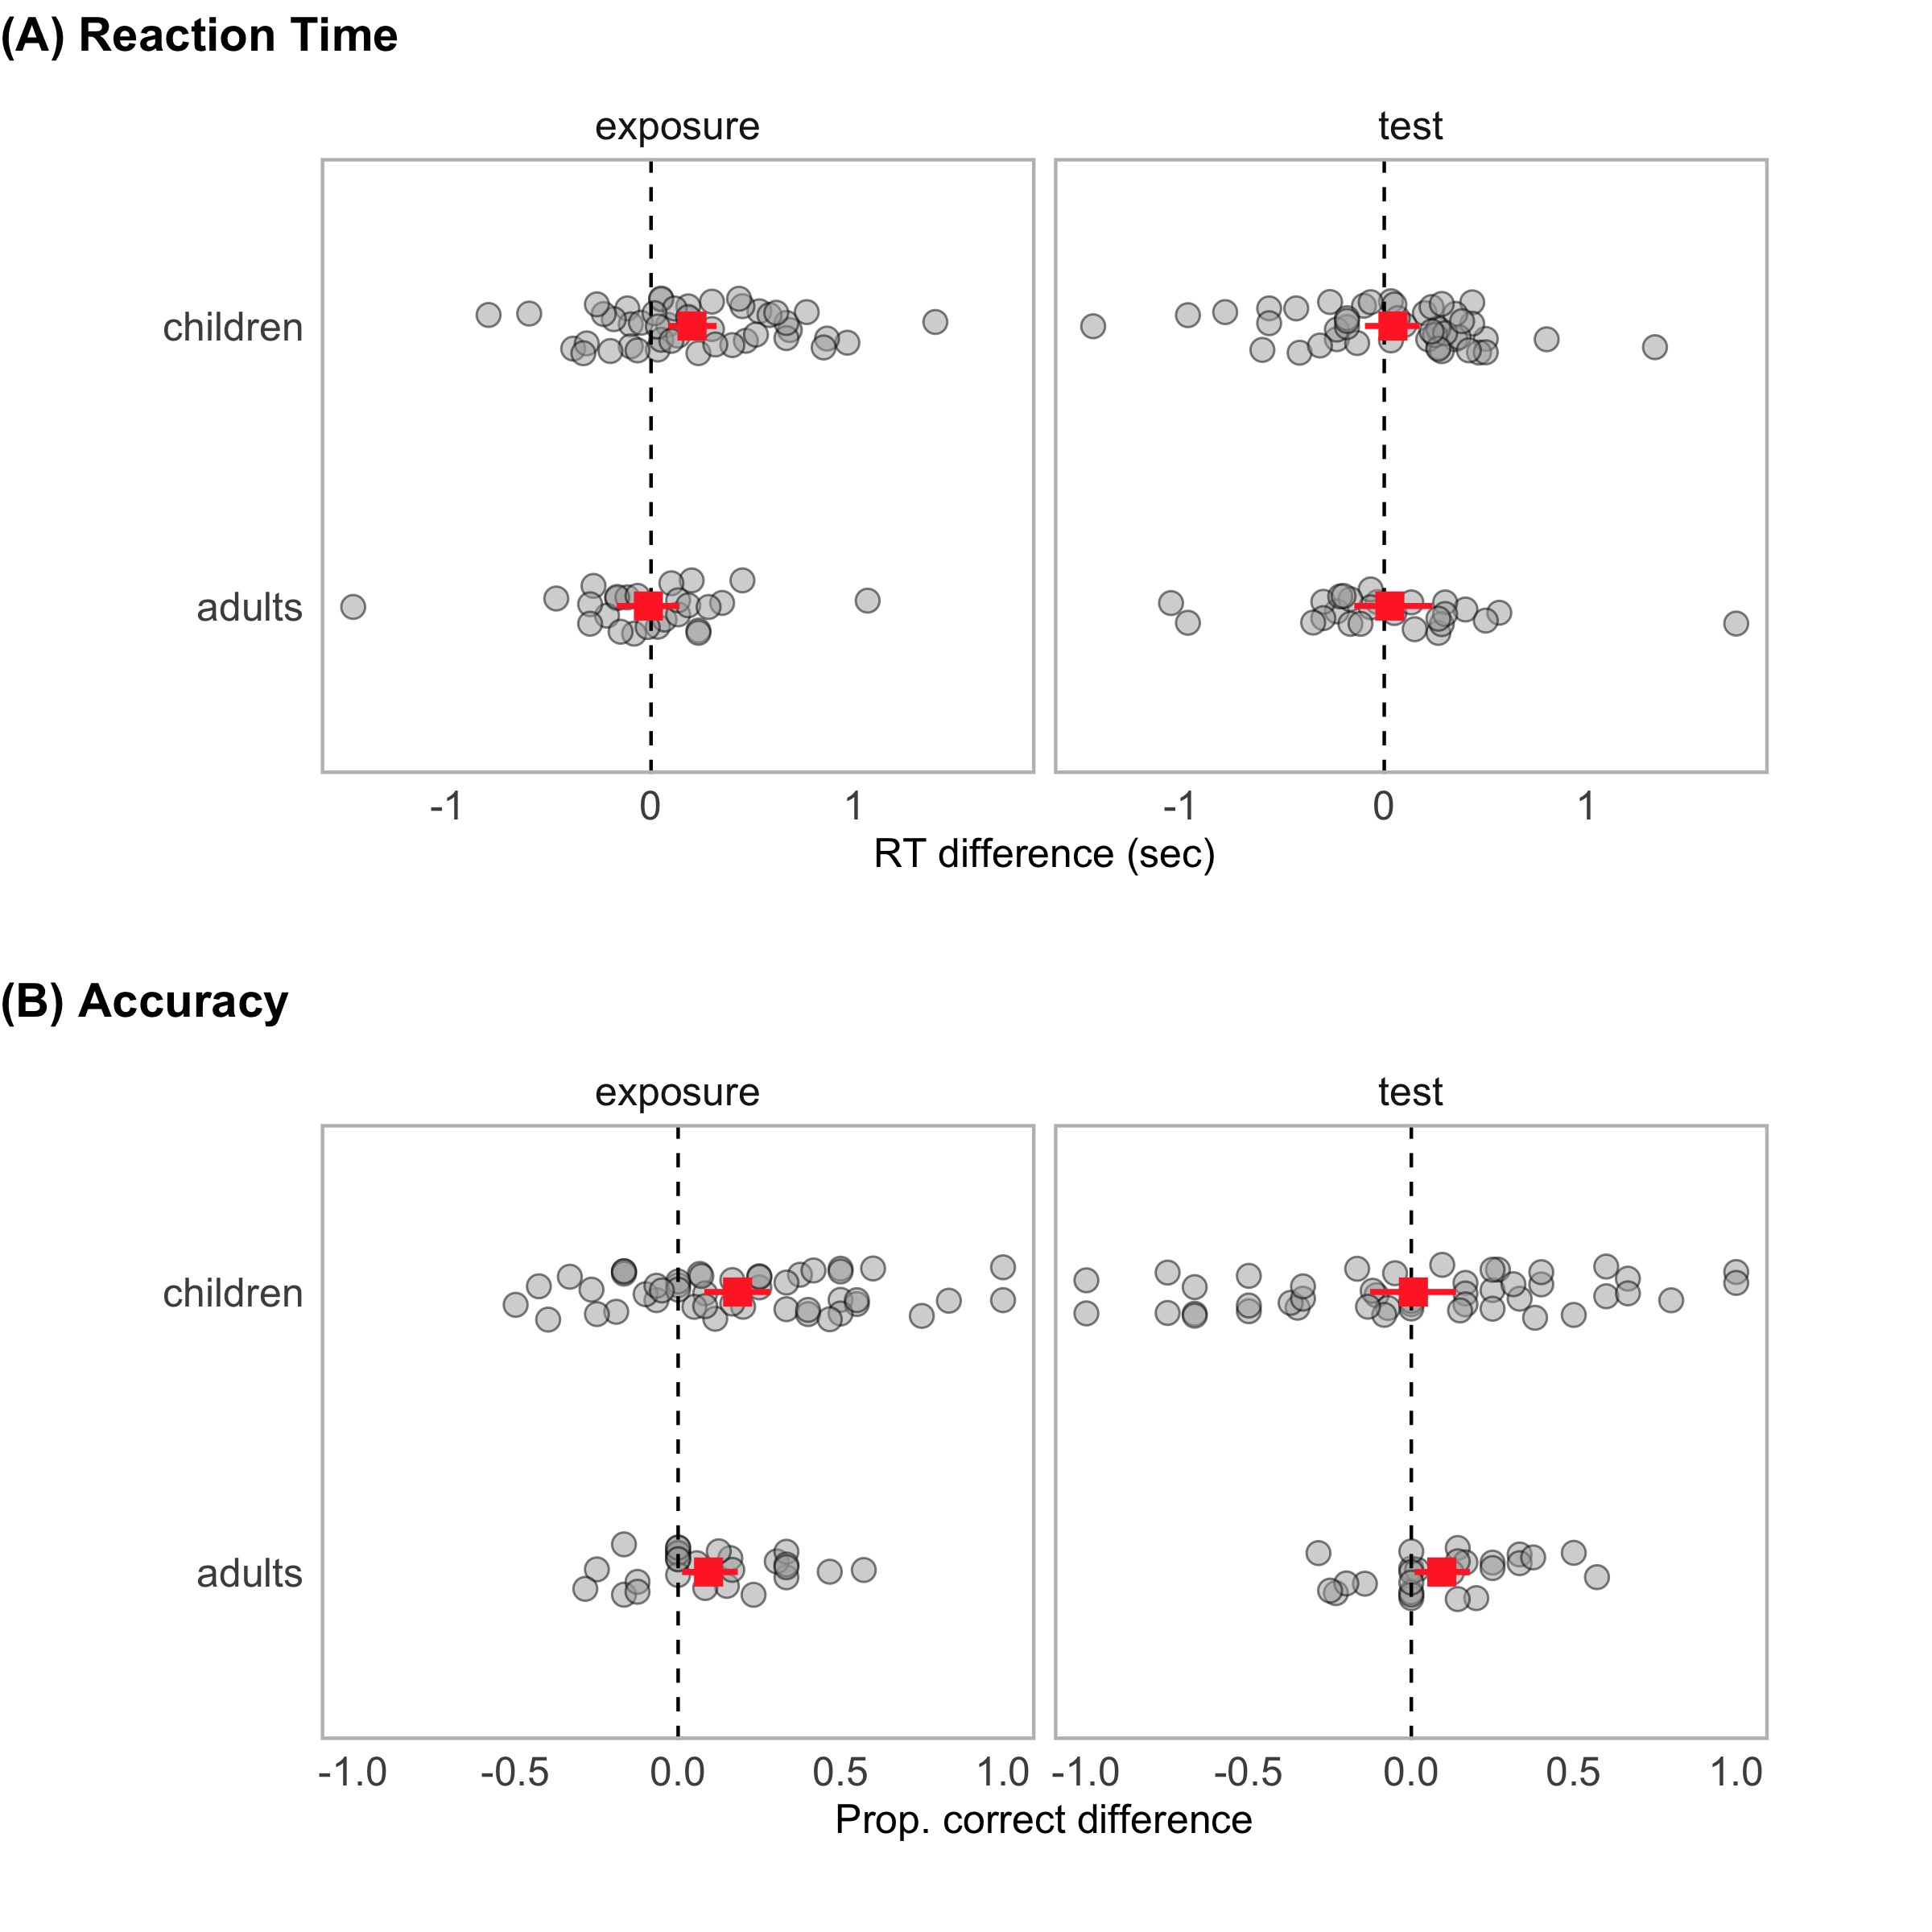
\includegraphics[width=0.8\linewidth]{/Users/kylemacdonald/Documents/Projects/SPEED-ACC-NOVEL/writing/figures/plots/speed_acc_novel_fstshifts} 

}

\caption{First shift Reaction Time (RT), and Accuracy results for children and adults in Experiment 3. Panel A shows the distribution of pairwise contrasts between RTs in the gaze and no-gaze conditions. The square point represents the mean value for each measure. The vertical dashed line represents the null model of zero condition difference. The width each point represents the 95\% HDI. Panel B shows the same information but for participants' first shift accuracy.}\label{fig:speed-acc-novel-shifts}
\end{figure}

We next asked how the presence of gaze influenced learners' decision to
stop gathering visual information from the speaker and start fixating on
the novel objects. To quantify the effect the gaze, we fit a Bayesian
linear mixed-effects regression predicting first shift RT as a function
of whether there was a gaze cue present on the trial and age group. Both
children (Gaze \(M_{rt}\) = 1,136.77 ms, No-gaze \(M_{rt}\) = 781.66 ms)
and adults (Gaze \(M_{rt}\) = 878.65 ms, No-gaze \(M_{rt}\) = 772.08 ms)
fixated longer on the speaker when she provided a gaze cue (\(\beta\) =
-0.25, 95\% HDI {[}-0.41, -0.09{]}). With no evidence of an interaction
between gaze condition and age group (\(\beta_{int}\) = 0.15, 95\% HDI
{[}-0.08, 0.39{]}). Moreover, both (Gaze \(M_{acc}\) = 0.64, No-gaze
\(M_{acc}\) = 0.49) and adults (Gaze \(M_{acc}\) = 0.89, No-gaze
\(M_{acc}\) = 0.81) generated more accurate first shifts in the gaze
condition, indicating they were following the gaze cue on Exposure
trials (\(\beta\) = -0.67, 95\% HDI {[}-1.11, -0.26{]}).

Finally, we asked whether the presence of gaze affected subsequent
learning by fitting the same accuracy model on Test trials. We found
that adults were much more accurate than children (\(\beta_{age}\) =
-0.93, 95\% HDI {[}-2.36, 0.44{]}), and that both children and adults
generated shifts that landed on the target with similar accuracy
regardless of whether the Test trial was preceded by an Exposure trial
with a gaze cue (\(\beta_{gaze}\) = -0.21, 95\% HDI {[}-0.91, 0.48{]}).

Overall, the first shift analyses provide converging, albeit mixed,
evidence that learners' modulated their decisions about visual fixation
to gather additional a post-nominal gaze cue when it was available.
Children but not adults generated slower first shifts away from a
speaker's face when there was a Gaze cue to gather. Both children and
adults generated a higher proportion of shifts landing on the target
image when there was post-nominal gaze cue available. Finally, adults,
but not children, generated more accurate first shifts on Test trials
that were preceded by Exposure trials with gaze. The absence of
condition differences for children's performance on Test trials
parallels the timecourse looking analyses and suggest that children were
not learning the novel word-object links well enough in either context.

\section{General Discussion}\label{general-discussion}

During grounded language processing, looks to a speaker or to objects
can faciliate comprehension and learning. Do children flexibly seek
visual information to support these goals? And how does information
seeking adapt as children gain more exposure to consistent word-object
pairings across multiple labeling events? In this work, we pursued the
idea that learners flexibly adapt their gaze to seek disambiguating
information from social partners when it is useful for their
comprehension and learning. We presented evidence for this explanation
by tracking children and adults' eye movements as they processed both
familiar and novel words accompanied by an ecologically-valid social cue
to reference (eye gaze). We also measured how gaze learners' gaze
dynamics changed as a function of accumulating statistical information
about the target word-object mappings.

In Experiment 1, we found that, children and adults showed parallel gaze
responses while processing familiar words, shifting attention away from
the speaker's face before she produced a post-nominal gaze cue.
Experiment 2 showed that the presence of gaze in the context of novel
objects focused adults' attention on a single object and modulated the
strength of the relationship between visual attention during labeling
and subsquent measures of recall for newly learned word-object pairs.
Finally, in Experiment 3, we found that both children and adults fixated
longer on a speaker who produced a gaze cue while labeling novel
objects, and this behavior led to more attention to the target object
and less looking to the distracter object. Both age groups, however,
were capable of learning the novel word-object pairings from
cross-situational stastics alone, and only adults showed evidence of
stronger learning in the less ambiguous context of social gaze.

\subsection{Limitations}\label{limitations-1}

This work has several important limitations. First, we did not see
evidence of that the effects of gaze generalized to learning
trajectories in children in Experiment 3. Moreover, we did not see
evidence of strong uptake of the novel word-object links overall. Our
future work is aimed at modifying the task to increase children's
learning and thus the opportunity to detect any effect of social
information over a longer timescale. For example, we plan to make the
social cue stronger by increasing the length of time the speaker gazed
at the object, which in the current stimulus set was relatively brief
social cue (\textasciitilde{}1 sec). We also plan to pair the
newly-learned novel objects against one another on Test trials, which
would reduce any attraction of novelty that pushed children to look at
the distracter object that they had not seen before on Test trials in
the current design.

Second, while we do measure the effects of social information on
learning over multiple labeling events, it is still a much shorter
timescale and smaller number of exposures relative to children's
ecological task. Moreover, the visual world paradigm, while
well-controlled, is highly constrained in terms of the complexity of
information seeking decisions that children make when allocating visual
attention in their naturalistic learning environments. Thus, a valuable
next step for this work would be to leverage tasks that move closer to
the ecological context in which children process and learn language such
as using head-mounted cameras and eye trackers that would allow
measurement of where children choose to look during everyday
interactions. It would be interesting to measure changes in children's
looking to communicative partners when they are first introduced to
novel objects in their day-to-day lives.

Third, we used a binary manipulation of the quality of information
available in the social context -- full disambiguating gaze cue or
totally ambiguous absence of a gaze cue -- which does not reflect the
complexity of children's social interactions. That is, children's social
partners are more likely to provide intermediate levels of
disambiguating information during novel object labeling. Morever, our
prior work suggests that adults are sensitive to the graded changes in
the reliability of a gaze cue, storing word-object links with greater
fidelity as reliability increased (MacDonald et al., 2017). Thus, it
seems useful to know how children's real-time information selection
responds to continuous changes in referential ambiguity.

\subsection{Conclusions}\label{conclusions}

In this paper, we presented a set of empirical studies that integrate
ideas from social-pragmatic and statistical accounts of language
acquisition. We found that listeners' decisions to wait and seek social
information depended on their uncertainty over the word-object mappings.
Only in the case of processing novel words did learners adapt their gaze
dynamics to seek a post-nominal social cue to reference. Moreover,
processing novel words with an available gaze cue modulated the
relationship between learners' real-time looking behavior during
labeling and retention at a longer timescale. More generally, this work
sheds light on how children can use eye movements as an active
information gathering process within social contexts, which, in turn,
shapes the information that comes into contact with their statistical
learning mechanisms.

\newpage

\section{References}\label{references}

\begingroup
\setlength{\parindent}{-0.5in} \setlength{\leftskip}{0.5in}

\hypertarget{refs}{}
\hypertarget{ref-allopenna1998tracking}{}
Allopenna, P. D., Magnuson, J. S., \& Tanenhaus, M. K. (1998). Tracking
the time course of spoken word recognition using eye movements: Evidence
for continuous mapping models. \emph{Journal of Memory and Language},
\emph{38}(4), 419--439.

\hypertarget{ref-baldwin1993infants}{}
Baldwin, D. A. (1993). Infants' ability to consult the speaker for clues
to word reference. \emph{Journal of Child Language}, \emph{20}(02),
395--418.

\hypertarget{ref-bloom2002children}{}
Bloom, P. (2002). \emph{How children learn the meaning of words}. The
MIT Press.

\hypertarget{ref-blythe2016word}{}
Blythe, R. A., Smith, A. D., \& Smith, K. (2016). Word learning under
infinite uncertainty. \emph{Cognition}, \emph{151}, 18--27.

\hypertarget{ref-blythe2010learning}{}
Blythe, R. A., Smith, K., \& Smith, A. D. (2010). Learning times for
large lexicons through cross-situational learning. \emph{Cognitive
Science}, \emph{34}(4), 620--642.

\hypertarget{ref-brooks2005development}{}
Brooks, R., \& Meltzoff, A. N. (2005). The development of gaze following
and its relation to language. \emph{Developmental Science}, \emph{8}(6),
535--543.

\hypertarget{ref-burkner2017brms}{}
Bürkner, P.-C., \& others. (2017). Brms: An r package for bayesian
multilevel models using stan. \emph{Journal of Statistical Software},
\emph{80}(1), 1--28.

\hypertarget{ref-carpenter1998social}{}
Carpenter, M., Nagell, K., Tomasello, M., Butterworth, G., \& Moore, C.
(1998). Social cognition, joint attention, and communicative competence
from 9 to 15 months of age. \emph{Monographs of the Society for Research
in Child Development}, i--174.

\hypertarget{ref-castro2009human}{}
Castro, R. M., Kalish, C., Nowak, R., Qian, R., Rogers, T., \& Zhu, X.
(2009). Human active learning. In \emph{Advances in neural information
processing systems} (pp. 241--248).

\hypertarget{ref-clark2009first}{}
Clark, E. V. (2009). \emph{First language acquisition}. Cambridge
University Press.

\hypertarget{ref-estigarribia2007getting}{}
Estigarribia, B., \& Clark, E. V. (2007). Getting and maintaining
attention in talk to young children. \emph{Journal of Child Language},
\emph{34}(4), 799--814.

\hypertarget{ref-frank2009using}{}
Frank, M. C., Goodman, N. D., \& Tenenbaum, J. B. (2009). Using
speakers' referential intentions to model early cross-situational word
learning. \emph{Psychological Science}, \emph{20}(5), 578--585.

\hypertarget{ref-gureckis2012self}{}
Gureckis, T. M., \& Markant, D. B. (2012). Self-directed learning a
cognitive and computational perspective. \emph{Perspectives on
Psychological Science}, \emph{7}(5), 464--481.

\hypertarget{ref-hayhoe2005eye}{}
Hayhoe, M., \& Ballard, D. (2005). Eye movements in natural behavior.
\emph{Trends in Cognitive Sciences}, \emph{9}(4), 188--194.

\hypertarget{ref-hidaka2017quantifying}{}
Hidaka, S., Torii, T., \& Kachergis, G. (2017). Quantifying the impact
of active choice in word learning. In. Cognitive Science Society.

\hypertarget{ref-hollich2000breaking}{}
Hollich, G. J., Hirsh-Pasek, K., Golinkoff, R. M., Brand, R. J., Brown,
E., Chung, H. L., \ldots{} Bloom, L. (2000). Breaking the language
barrier: An emergentist coalition model for the origins of word
learning. \emph{Monographs of the Society for Research in Child
Development}, i--135.

\hypertarget{ref-kachergis2013actively}{}
Kachergis, G., Yu, C., \& Shiffrin, R. M. (2013). Actively learning
object names across ambiguous situations. \emph{Topics in Cognitive
Science}, \emph{5}(1), 200--213.

\hypertarget{ref-liszkowski2012prelinguistic}{}
Liszkowski, U., Brown, P., Callaghan, T., Takada, A., \& De Vos, C.
(2012). A prelinguistic gestural universal of human communication.
\emph{Cognitive Science}, \emph{36}(4), 698--713.

\hypertarget{ref-macdonald2018speed}{}
MacDonald, K., Marchman, V., Fernald, A., \& Frank, M. C. (2018).
Children seek visual information during signed and spoken language
comprehension. \emph{Preprint PsyArXiv}.

\hypertarget{ref-macdonald2017social}{}
MacDonald, K., Yurovsky, D., \& Frank, M. C. (2017). Social cues
modulate the representations underlying cross-situational learning.
\emph{Cognitive Psychology}, \emph{94}, 67--84.

\hypertarget{ref-maris2007nonparametric}{}
Maris, E., \& Oostenveld, R. (2007). Nonparametric statistical testing
of eeg-and meg-data. \emph{Journal of Neuroscience Methods},
\emph{164}(1), 177--190.

\hypertarget{ref-mcmurray2012word}{}
McMurray, B., Horst, J. S., \& Samuelson, L. K. (2012). Word learning
emerges from the interaction of online referent selection and slow
associative learning. \emph{Psychological Review}, \emph{119}(4), 831.

\hypertarget{ref-partridge2015young}{}
Partridge, E., McGovern, M. G., Yung, A., \& Kidd, C. (2015). Young
children's self-directed information gathering on touchscreens. In
\emph{Proceedings of the 37th annual conference of the cognitive science
society}.

\hypertarget{ref-quine19600}{}
Quine, W. V. (1960). 0. word and object. \emph{111e MIT Press}.

\hypertarget{ref-ratcliff2015individual}{}
Ratcliff, R., \& Childers, R. (2015). Individual differences and fitting
methods for the two-choice diffusion model of decision making.
\emph{Decision}, \emph{2}(4), 237--279.

\hypertarget{ref-roy2002learning}{}
Roy, D. K., \& Pentland, A. P. (2002). Learning words from sights and
sounds: A computational model. \emph{Cognitive Science}, \emph{26}(1),
113--146.

\hypertarget{ref-settles2012active}{}
Settles, B. (2012). Active learning. \emph{Synthesis Lectures on
Artificial Intelligence and Machine Learning}, \emph{6}(1), 1--114.

\hypertarget{ref-siskind1996computational}{}
Siskind, J. M. (1996). A computational study of cross-situational
techniques for learning word-to-meaning mappings. \emph{Cognition},
\emph{61}(1), 39--91.

\hypertarget{ref-smith2008infants}{}
Smith, L. B., \& Yu, C. (2008). Infants rapidly learn word-referent
mappings via cross-situational statistics. \emph{Cognition},
\emph{106}(3), 1558--1568.

\hypertarget{ref-smith2013visual}{}
Smith, L. B., \& Yu, C. (2013). Visual attention is not enough:
Individual differences in statistical word-referent learning in infants.
\emph{Language Learning and Development}, \emph{9}(1), 25--49.

\hypertarget{ref-yu2007unified}{}
Yu, C., \& Ballard, D. H. (2007). A unified model of early word
learning: Integrating statistical and social cues.
\emph{Neurocomputing}, \emph{70}(13), 2149--2165.

\hypertarget{ref-yu2007rapid}{}
Yu, C., \& Smith, L. B. (2007). Rapid word learning under uncertainty
via cross-situational statistics. \emph{Psychological Science},
\emph{18}(5), 414--420.

\endgroup


\end{document}
